%%%%%%%PACKAGES%%%%%%%
    \documentclass[11pt,twoside,openany]{memoir}
    \usepackage[T1]{fontenc}
    \usepackage[utf8]{inputenc}
    \usepackage{titlesec}
    \usepackage{anyfontsize}
    \usepackage{fancybox}
    \usepackage[dvipsnames,svgnames,x11names,hyperref]{xcolor}
    \usepackage{enumerate}
    \usepackage{comment}
    \usepackage{amsfonts}
    \usepackage{amsthm}
    \usepackage{amsmath}
    \usepackage{amssymb}
    \usepackage{hyperref}
    \usepackage{fullpage}
    \usepackage{bm}
    \usepackage{cprotect}
    \usepackage{calligra}
    \usepackage{emptypage}
    \usepackage{titleps}
    \usepackage{microtype}
    \usepackage{float}
    \usepackage{ocgx}
    \usepackage{appendix}
    \usepackage{graphicx}
    \usepackage{pdfcomment}
    \usepackage{enumitem}
    \usepackage{mathtools}
    \usepackage{tikz-cd}
    \usepackage{relsize}
    \usepackage[font=footnotesize,labelfont=bf]{caption}
    \usepackage{changepage}
    \usepackage{xcolor}
    \usepackage{ulem}
    \usepackage{marginnote}
        \newcommand*{\mnote}[1]{ % <----------
        \checkoddpage
        \ifoddpage
            \marginparmargin{left}
        \else
            \marginparmargin{right}
        \fi
            \marginnote{\tiny \textcolor{oorange}{#1}}
        }
    \usepackage{tgbonum}
    \usepackage{datetime}
        \newdateformat{specialdate}{\THEYEAR\ \monthname\ \THEDAY}
    \usepackage[margin=0.9in]{geometry}
        \setlength{\voffset}{-0.4in}
        \setlength{\headsep}{30pt}
    \usepackage{fancyhdr}
        \fancyhf{}
        \pagestyle{fancy}
        \cfoot{\footnotesize \thepage}
        \fancyhead[R]{\footnotesize \rightmark}
        \fancyhead[L]{\footnotesize \leftmark}
    \usepackage[T1]{fontenc}% http://ctan.org/pkg/fontenc
    \usepackage[outline]{contour}% http://ctan.org/pkg/contour
        \renewcommand{\arraystretch}{1.5}
        \contourlength{0.4pt}
        \contournumber{10}%
    \usepackage{letterspace}







    

%%%%%%%%%%%%%%%%%%%%%%
%%%%%%%%MACROS%%%%%%%%
%%%%%%%%%%%%%%%%%%%%%%
    %to make the correct symbol for Sha
%\newcommand\cyr{%
%\renewcommand\rmdefault{wncyr}%
%\renewcommand\sfdefault{wncyss}%
%\renewcommand\encodingdefault{OT2}%
%\normalfont \selectfont} \DeclareTextFontCommand{\textcyr}{\cyr}


\DeclareMathOperator{\ab}{ab}
\newcommand{\absgal}{\G_{\bbQ}}
\DeclareMathOperator{\ad}{ad}
\DeclareMathOperator{\adj}{adj}
\DeclareMathOperator{\alg}{alg}
\DeclareMathOperator{\Alt}{Alt}
\DeclareMathOperator{\Ann}{Ann}
\DeclareMathOperator{\arith}{arith}
\DeclareMathOperator{\Aut}{Aut}
\DeclareMathOperator{\Be}{B}
\DeclareMathOperator{\card}{card}
\DeclareMathOperator{\Char}{char}
\DeclareMathOperator{\csp}{csp}
\DeclareMathOperator{\codim}{codim}
\DeclareMathOperator{\coker}{coker}
\DeclareMathOperator{\coh}{H}
\DeclareMathOperator{\compl}{compl}
\DeclareMathOperator{\conj}{conj}
\DeclareMathOperator{\cont}{cont}
\DeclareMathOperator{\crys}{crys}
\DeclareMathOperator{\Crys}{Crys}
\DeclareMathOperator{\cusp}{cusp}
\DeclareMathOperator{\diag}{diag}
\DeclareMathOperator{\disc}{disc}
\DeclareMathOperator{\dR}{dR}
\DeclareMathOperator{\Eis}{Eis}
\DeclareMathOperator{\End}{End}
\DeclareMathOperator{\ev}{ev}
\DeclareMathOperator{\eval}{eval}
\DeclareMathOperator{\Eq}{Eq}
\DeclareMathOperator{\Ext}{Ext}
\DeclareMathOperator{\Fil}{Fil}
\DeclareMathOperator{\Fitt}{Fitt}
\DeclareMathOperator{\Frob}{Frob}
\DeclareMathOperator{\G}{G}
\DeclareMathOperator{\Gal}{Gal}
\DeclareMathOperator{\GL}{GL}
\DeclareMathOperator{\Gr}{Gr}
\DeclareMathOperator{\Graph}{Graph}
\DeclareMathOperator{\GSp}{GSp}
\DeclareMathOperator{\GUn}{GU}
\DeclareMathOperator{\Hom}{Hom}
\DeclareMathOperator{\id}{id}
\DeclareMathOperator{\Id}{Id}
\DeclareMathOperator{\Ik}{Ik}
\DeclareMathOperator{\IM}{Im}
\DeclareMathOperator{\Image}{im}
\DeclareMathOperator{\Ind}{Ind}
\DeclareMathOperator{\Inf}{inf}
\DeclareMathOperator{\Isom}{Isom}
\DeclareMathOperator{\J}{J}
\DeclareMathOperator{\Jac}{Jac}
\DeclareMathOperator{\lcm}{lcm}
\DeclareMathOperator{\length}{length}
\DeclareMathOperator{\Log}{Log}
\DeclareMathOperator{\M}{M}
\DeclareMathOperator{\Mat}{Mat}
\DeclareMathOperator{\N}{N}
\DeclareMathOperator{\Nm}{Nm}
\DeclareMathOperator{\NIk}{N-Ik}
\DeclareMathOperator{\NSK}{N-SK}
\DeclareMathOperator{\new}{new}
\DeclareMathOperator{\obj}{obj}
\DeclareMathOperator{\old}{old}
\DeclareMathOperator{\ord}{ord}
\DeclareMathOperator{\Or}{O}
\DeclareMathOperator{\PGL}{PGL}
\DeclareMathOperator{\PGSp}{PGSp}
\DeclareMathOperator{\rank}{rank}
\DeclareMathOperator{\Rel}{Rel}
\DeclareMathOperator{\Real}{Re}
\DeclareMathOperator{\RES}{res}
\DeclareMathOperator{\Res}{Res}
%\DeclareMathOperator{\Sha}{\textcyr{Sh}}
\DeclareMathOperator{\Sel}{Sel}
\DeclareMathOperator{\semi}{ss}
\DeclareMathOperator{\sgn}{sign}
\DeclareMathOperator{\SK}{SK}
\DeclareMathOperator{\SL}{SL}
\DeclareMathOperator{\SO}{SO}
\DeclareMathOperator{\Sp}{Sp}
\DeclareMathOperator{\Span}{span}
\DeclareMathOperator{\Spec}{Spec}
\DeclareMathOperator{\spin}{spin}
\DeclareMathOperator{\st}{st}
\DeclareMathOperator{\St}{St}
\DeclareMathOperator{\SUn}{SU}
\DeclareMathOperator{\supp}{supp}
\DeclareMathOperator{\Sup}{sup}
\DeclareMathOperator{\Sym}{Sym}
\DeclareMathOperator{\Tam}{Tam}
\DeclareMathOperator{\tors}{tors}
\DeclareMathOperator{\tr}{tr}
\DeclareMathOperator{\un}{un}
\DeclareMathOperator{\Un}{U}
\DeclareMathOperator{\val}{val}
\DeclareMathOperator{\vol}{vol}

\DeclareMathOperator{\Sets}{S \mkern1.04mu e \mkern1.04mu t \mkern1.04mu s}
    \newcommand{\cSets}{\scalebox{1.02}{\contour{black}{$\Sets$}}}
    
\DeclareMathOperator{\Groups}{G \mkern1.04mu r \mkern1.04mu o \mkern1.04mu u \mkern1.04mu p \mkern1.04mu s}
    \newcommand{\cGroups}{\scalebox{1.02}{\contour{black}{$\Groups$}}}

\DeclareMathOperator{\TTop}{T \mkern1.04mu o \mkern1.04mu p}
    \newcommand{\cTop}{\scalebox{1.02}{\contour{black}{$\TTop$}}}

\DeclareMathOperator{\Htp}{H \mkern1.04mu t \mkern1.04mu p}
    \newcommand{\cHtp}{\scalebox{1.02}{\contour{black}{$\Htp$}}}

\DeclareMathOperator{\Mod}{M \mkern1.04mu o \mkern1.04mu d}
    \newcommand{\cMod}{\scalebox{1.02}{\contour{black}{$\Mod$}}}

\DeclareMathOperator{\Ab}{A \mkern1.04mu b}
    \newcommand{\cAb}{\scalebox{1.02}{\contour{black}{$\Ab$}}}

\DeclareMathOperator{\Rings}{R \mkern1.04mu i \mkern1.04mu n \mkern1.04mu g \mkern1.04mu s}
    \newcommand{\cRings}{\scalebox{1.02}{\contour{black}{$\Rings$}}}

\DeclareMathOperator{\ComRings}{C \mkern1.04mu o \mkern1.04mu m \mkern1.04mu R \mkern1.04mu i \mkern1.04mu n \mkern1.04mu g \mkern1.04mu s}
    \newcommand{\cComRings}{\scalebox{1.05}{\contour{black}{$\ComRings$}}}

\DeclareMathOperator{\hHom}{H \mkern1.04mu o \mkern1.04mu m}
    \newcommand{\cHom}{\scalebox{1.02}{\contour{black}{$\hHom$}}}

         %  \item $\cGroups$
          %  \item $\cTop$
          %  \item $\cHtp$
          %  \item $\cMod$




\renewcommand{\k}{\kappa}
\newcommand{\Ff}{F_{f}}
\newcommand{\ts}{\,^{t}\!}


%Mathcal

\newcommand{\cA}{\mathcal{A}}
\newcommand{\cB}{\mathcal{B}}
\newcommand{\cC}{\mathcal{C}}
\newcommand{\cD}{\mathcal{D}}
\newcommand{\cE}{\mathcal{E}}
\newcommand{\cF}{\mathcal{F}}
\newcommand{\cG}{\mathcal{G}}
\newcommand{\cH}{\mathcal{H}}
\newcommand{\cI}{\mathcal{I}}
\newcommand{\cJ}{\mathcal{J}}
\newcommand{\cK}{\mathcal{K}}
\newcommand{\cL}{\mathcal{L}}
\newcommand{\cM}{\mathcal{M}}
\newcommand{\cN}{\mathcal{N}}
\newcommand{\cO}{\mathcal{O}}
\newcommand{\cP}{\mathcal{P}}
\newcommand{\cQ}{\mathcal{Q}}
\newcommand{\cR}{\mathcal{R}}
\newcommand{\cS}{\mathcal{S}}
\newcommand{\cT}{\mathcal{T}}
\newcommand{\cU}{\mathcal{U}}
\newcommand{\cV}{\mathcal{V}}
\newcommand{\cW}{\mathcal{W}}
\newcommand{\cX}{\mathcal{X}}
\newcommand{\cY}{\mathcal{Y}}
\newcommand{\cZ}{\mathcal{Z}}


%mathfrak (missing \fi)

\newcommand{\fa}{\mathfrak{a}}
\newcommand{\fA}{\mathfrak{A}}
\newcommand{\fb}{\mathfrak{b}}
\newcommand{\fB}{\mathfrak{B}}
\newcommand{\fc}{\mathfrak{c}}
\newcommand{\fC}{\mathfrak{C}}
\newcommand{\fd}{\mathfrak{d}}
\newcommand{\fD}{\mathfrak{D}}
\newcommand{\fe}{\mathfrak{e}}
\newcommand{\fE}{\mathfrak{E}}
\newcommand{\ff}{\mathfrak{f}}
\newcommand{\fF}{\mathfrak{F}}
\newcommand{\fg}{\mathfrak{g}}
\newcommand{\fG}{\mathfrak{G}}
\newcommand{\fh}{\mathfrak{h}}
\newcommand{\fH}{\mathfrak{H}}
\newcommand{\fI}{\mathfrak{I}}
\newcommand{\fj}{\mathfrak{j}}
\newcommand{\fJ}{\mathfrak{J}}
\newcommand{\fk}{\mathfrak{k}}
\newcommand{\fK}{\mathfrak{K}}
\newcommand{\fl}{\mathfrak{l}}
\newcommand{\fL}{\mathfrak{L}}
\newcommand{\fm}{\mathfrak{m}}
\newcommand{\fM}{\mathfrak{M}}
\newcommand{\fn}{\mathfrak{n}}
\newcommand{\fN}{\mathfrak{N}}
\newcommand{\fo}{\mathfrak{o}}
\newcommand{\fO}{\mathfrak{O}}
\newcommand{\fp}{\mathfrak{p}}
\newcommand{\fP}{\mathfrak{P}}
\newcommand{\fq}{\mathfrak{q}}
\newcommand{\fQ}{\mathfrak{Q}}
\newcommand{\fr}{\mathfrak{r}}
\newcommand{\fR}{\mathfrak{R}}
\newcommand{\fs}{\mathfrak{s}}
\newcommand{\fS}{\mathfrak{S}}
\newcommand{\ft}{\mathfrak{t}}
\newcommand{\fT}{\mathfrak{T}}
\newcommand{\fu}{\mathfrak{u}}
\newcommand{\fU}{\mathfrak{U}}
\newcommand{\fv}{\mathfrak{v}}
\newcommand{\fV}{\mathfrak{V}}
\newcommand{\fw}{\mathfrak{w}}
\newcommand{\fW}{\mathfrak{W}}
\newcommand{\fx}{\mathfrak{x}}
\newcommand{\fX}{\mathfrak{X}}
\newcommand{\fy}{\mathfrak{y}}
\newcommand{\fY}{\mathfrak{Y}}
\newcommand{\fz}{\mathfrak{z}}
\newcommand{\fZ}{\mathfrak{Z}}


%mathbf

\newcommand{\bfA}{\mathbf{A}}
\newcommand{\bfB}{\mathbf{B}}
\newcommand{\bfC}{\mathbf{C}}
\newcommand{\bfD}{\mathbf{D}}
\newcommand{\bfE}{\mathbf{E}}
\newcommand{\bfF}{\mathbf{F}}
\newcommand{\bfG}{\mathbf{G}}
\newcommand{\bfH}{\mathbf{H}}
\newcommand{\bfI}{\mathbf{I}}
\newcommand{\bfJ}{\mathbf{J}}
\newcommand{\bfK}{\mathbf{K}}
\newcommand{\bfL}{\mathbf{L}}
\newcommand{\bfM}{\mathbf{M}}
\newcommand{\bfN}{\mathbf{N}}
\newcommand{\bfO}{\mathbf{O}}
\newcommand{\bfP}{\mathbf{P}}
\newcommand{\bfQ}{\mathbf{Q}}
\newcommand{\bfR}{\mathbf{R}}
\newcommand{\bfS}{\mathbf{S}}
\newcommand{\bfT}{\mathbf{T}}
\newcommand{\bfU}{\mathbf{U}}
\newcommand{\bfV}{\mathbf{V}}
\newcommand{\bfW}{\mathbf{W}}
\newcommand{\bfX}{\mathbf{X}}
\newcommand{\bfY}{\mathbf{Y}}
\newcommand{\bfZ}{\mathbf{Z}}

\newcommand{\bfa}{\mathbf{a}}
\newcommand{\bfb}{\mathbf{b}}
\newcommand{\bfc}{\mathbf{c}}
\newcommand{\bfd}{\mathbf{d}}
\newcommand{\bfe}{\mathbf{e}}
\newcommand{\bff}{\mathbf{f}}
\newcommand{\bfg}{\mathbf{g}}
\newcommand{\bfh}{\mathbf{h}}
\newcommand{\bfi}{\mathbf{i}}
\newcommand{\bfj}{\mathbf{j}}
\newcommand{\bfk}{\mathbf{k}}
\newcommand{\bfl}{\mathbf{l}}
\newcommand{\bfm}{\mathbf{m}}
\newcommand{\bfn}{\mathbf{n}}
\newcommand{\bfo}{\mathbf{o}}
\newcommand{\bfp}{\mathbf{p}}
\newcommand{\bfq}{\mathbf{q}}
\newcommand{\bfr}{\mathbf{r}}
\newcommand{\bfs}{\mathbf{s}}
\newcommand{\bft}{\mathbf{t}}
\newcommand{\bfu}{\mathbf{u}}
\newcommand{\bfv}{\mathbf{v}}
\newcommand{\bfw}{\mathbf{w}}
\newcommand{\bfx}{\mathbf{x}}
\newcommand{\bfy}{\mathbf{y}}
\newcommand{\bfz}{\mathbf{z}}

%blackboard bold

\newcommand{\bbA}{\mathbb{A}}
\newcommand{\bbB}{\mathbb{B}}
\newcommand{\bbC}{\mathbb{C}}
\newcommand{\bbD}{\mathbb{D}}
\newcommand{\bbE}{\mathbb{E}}
\newcommand{\bbF}{\mathbb{F}}
\newcommand{\bbG}{\mathbb{G}}
\newcommand{\bbH}{\mathbb{H}}
\newcommand{\bbI}{\mathbb{I}}
\newcommand{\bbJ}{\mathbb{J}}
\newcommand{\bbK}{\mathbb{K}}
\newcommand{\bbL}{\mathbb{L}}
\newcommand{\bbM}{\mathbb{M}}
\newcommand{\bbN}{\mathbb{N}}
\newcommand{\bbO}{\mathbb{O}}
\newcommand{\bbP}{\mathbb{P}}
\newcommand{\bbQ}{\mathbb{Q}}
\newcommand{\bbR}{\mathbb{R}}
\newcommand{\bbS}{\mathbb{S}}
\newcommand{\bbT}{\mathbb{T}}
\newcommand{\bbU}{\mathbb{U}}
\newcommand{\bbV}{\mathbb{V}}
\newcommand{\bbW}{\mathbb{W}}
\newcommand{\bbX}{\mathbb{X}}
\newcommand{\bbY}{\mathbb{Y}}
\newcommand{\bbZ}{\mathbb{Z}}

\newcommand{\bmat}{\left( \begin{matrix}}
\newcommand{\emat}{\end{matrix} \right)}

\newcommand{\pmat}{\left( \begin{smallmatrix}}
\newcommand{\epmat}{\end{smallmatrix} \right)}

\newcommand{\lat}{\mathscr{L}}
\newcommand{\mat}[4]{\begin{pmatrix}{#1}&{#2}\\{#3}&{#4}\end{pmatrix}}
\newcommand{\ov}[1]{\overline{#1}}
\newcommand{\res}[1]{\underset{#1}{\RES}\,}
\newcommand{\up}{\upsilon}

\newcommand{\tac}{\textasteriskcentered}

%mahesh macros
\newcommand{\tm}{\textrm}

%Comments
\newcommand{\com}[1]{\vspace{5 mm}\par \noindent
\marginpar{\textsc{Comment}} \framebox{\begin{minipage}[c]{0.95
\textwidth} \tt #1 \end{minipage}}\vspace{5 mm}\par}

\newcommand{\Bmu}{\mbox{$\raisebox{-0.59ex}
  {$l$}\hspace{-0.18em}\mu\hspace{-0.88em}\raisebox{-0.98ex}{\scalebox{2}
  {$\color{white}.$}}\hspace{-0.416em}\raisebox{+0.88ex}
  {$\color{white}.$}\hspace{0.46em}$}{}}  %need graphicx and xcolor. this produces blackboard bold mu 

\newcommand{\hooktwoheadrightarrow}{%
  \hookrightarrow\mathrel{\mspace{-15mu}}\rightarrow
}

\makeatletter
\newcommand{\xhooktwoheadrightarrow}[2][]{%
  \lhook\joinrel
  \ext@arrow 0359\rightarrowfill@ {#1}{#2}%
  \mathrel{\mspace{-15mu}}\rightarrow
}
\makeatother

\renewcommand{\geq}{\geqslant}
    \renewcommand{\leq}{\leqslant}
    
    \newcommand{\bone}{\mathbf{1}}
    \newcommand{\sign}{\mathrm{sign}}
    \newcommand{\eps}{\varepsilon}
    \newcommand{\textui}[1]{\uline{\textit{#1}}}
    
    %\newcommand{\ov}{\overline}
    %\newcommand{\un}{\underline}
    \newcommand{\fin}{\mathrm{fin}}
    
    \newcommand{\chnum}{\titleformat
    {\chapter} % command
    [display] % shape
    {\centering} % format
    {\Huge \color{black} \shadowbox{\thechapter}} % label
    {-0.5em} % sep (space between the number and title)
    {\LARGE \color{black} \underline} % before-code
    }
    
    \newcommand{\chunnum}{\titleformat
    {\chapter} % command
    [display] % shape
    {} % format
    {} % label
    {0em} % sep
    { \begin{flushright} \begin{tabular}{r}  \Huge \color{black}
    } % before-code
    [
    \end{tabular} \end{flushright} \normalsize
    ] % after-code
    }

\newcommand{\littletaller}{\mathchoice{\vphantom{\big|}}{}{}{}}
\newcommand\restr[2]{{% we make the whole thing an ordinary symbol
  \left.\kern-\nulldelimiterspace % automatically resize the bar with \right
  #1 % the function
  \littletaller % pretend it's a little taller at normal size
  \right|_{#2} % this is the delimiter
  }}

\newcommand{\mtext}[1]{\hspace{6pt}\text{#1}\hspace{6pt}}

%This adds a "front cover" page.
%{\thispagestyle{empty}
%\vspace*{\fill}
%\begin{tabular}{l}
%\begin{tabular}{l}
%\includegraphics[scale=0.24]{oxy-logo.png}
%\end{tabular} \\
%\begin{tabular}{l}
%\Large \color{black} Module Theory, Linear Algebra, and Homological Algebra \\ \Large \color{black} Gianluca Crescenzo
%\end{tabular}
%\end{tabular}
%\newpage

    \newcommand{\TBC}{\textbf{TO BE CONTINUED}}
    \theoremstyle{plain}
    \newtheorem{theorem}{Theorem}[section]
    \newtheorem{proposition}[theorem]{Proposition}
    \newtheorem{corollary}[theorem]{Corollary}
    \newtheorem{lemma}[theorem]{Lemma}
    \newtheorem{open}[theorem]{Open problem}
    \newtheorem{fact}[theorem]{Fact}
    
    \theoremstyle{definition}
    \newtheorem{definition}[theorem]{Definition}
    \newtheorem*{definition*}{Definition}
    \newtheorem{example}{Example}[section]
    \newtheorem{notation}[theorem]{Notation}
    \newtheorem{exercise}{Exercise}[chapter]
    \newtheorem{practice}[exercise]{Practice}
    \newtheorem{challenge}[exercise]{Challenge}
    \newtheorem{homework}{Homework}
    \newtheorem{note}{Note}[section]
    
    \theoremstyle{remark}
    \newtheorem{remark}[theorem]{Remark}
    \newtheorem*{noproof}{Proof omitted}
    \numberwithin{equation}{section}
    
    \newenvironment{solution}[1]{\noindent \textbf{#1}:}{}
    
    \newcommand{\NN}{\mathbf{N}}
    \newcommand{\ZZ}{\mathbf{Z}}
    \newcommand{\QQ}{\mathbf{Q}}
    \newcommand{\RR}{\mathbf{R}}
    \newcommand{\CC}{\mathbf{C}}
    \newcommand{\HH}{\mathbf{H}}
    \newcommand{\KK}{\mathbf{K}}
    \newcommand{\FF}{\mathbf{F}}
    
    \newcommand{\bRR}{\overline{\RR}}
    \newcommand{\bRRp}{\overline{\RR}_{\geq 0}}
    
    \renewcommand{\geq}{\geqslant}
    \renewcommand{\leq}{\leqslant}
    
    \newcommand{\cA}{\mathcal{A}}
    \newcommand{\cB}{\mathcal{B}}
    \newcommand{\cC}{\mathcal{C}}
    \newcommand{\cF}{\mathcal{F}}
    \newcommand{\cL}{\mathcal{L}}
    \newcommand{\cM}{\mathcal{M}}
    \newcommand{\cN}{\mathcal{N}}
    \newcommand{\cU}{\mathcal{U}}
    \newcommand{\bone}{\mathbf{1}}
    \newcommand{\sign}{\mathrm{sign}}
    \newcommand{\eps}{\varepsilon}
    \newcommand{\textui}[1]{\uline{\textit{#1}}}
    
    %\newcommand{\ov}{\overline}
    %\newcommand{\un}{\underline}
    \newcommand{\fin}{\mathrm{fin}}
    
    \newcommand{\chnum}{\titleformat
    {\chapter} % command
    [display] % shape
    {} % format
    {} % label
    {-8em} % sep
    { \begin{flushright} \begin{tabular}{r} \fontsize{55}{20}\selectfont \color{black} \shadowbox{\thechapter} \\ \Huge \color{black}
    } % before-code
    [
    \end{tabular} \end{flushright} \normalsize
    ] % after-code
    }
    
    \newcommand{\chunnum}{\titleformat
    {\chapter} % command
    [display] % shape
    {} % format
    {} % label
    {0em} % sep
    { \begin{flushright} \begin{tabular}{r}  \Huge \color{black}
    } % before-code
    [
    \end{tabular} \end{flushright} \normalsize
    ] % after-code
    }





    
%%%%%%%%%%%%%%%%%%%%%%
%%%%DOCUMENT SETUP%%%%
%%%%%%%%%%%%%%%%%%%%%%
    \setsecnumdepth{subsection}
    \definecolor{bluey}{RGB}{21, 80, 234}
    \definecolor{darkgreen}{rgb}{0, 0.5976, 0}
    \hypersetup{pdfauthor=Gianluca Crescenzo, pdftitle=Rotman's Notes, pdfstartview=FitH, colorlinks=true, linkcolor=darkgreen, citecolor=darkgreen}
    
    \begin{document}
    
    %This adds a "front cover" page.
    %{\thispagestyle{empty}
    %\vspace*{\fill}
    %\begin{tabular}{l}
    %\begin{tabular}{l}
    %\includegraphics[scale=0.24]{oxy-logo.png}
    %\end{tabular} \\
    %\begin{tabular}{l}
    %\Large \color{black} Module Theory, Linear Algebra, and Homological Algebra \\ \Large \color{black} Gianluca Crescenzo
    %\end{tabular}
    %\end{tabular}
    
    %\newpage
    \pagenumbering{roman}
    \tableofcontents
    
    \chunnum
    \vfill
    \specialdate
    Last update: \today
    \chnum

    \chapter{Introduction}\label{chapter:introduction}

\pagenumbering{arabic}

\section{Simplicial Homology}\label{sec:simplicial-homology-sec}
    \begin{definition}\label{def:simplex}
        An \textui{$n$-simplex} is an $n$-dimensional geometric object with flat sides\footnote{Another word for this is a \textui{polytope}} that is convex hull; i.e., it is the smallest "shape" that encloses "everything" without a concavity.
    \end{definition}

    \begin{example}
        \phantom{a}
        \begin{enumerate}
            \item A $0$-dimensional simplex is a point.
            \item A $1$-dimensional simplex is a line.
            \item A $2$-dimensional simplex is a triangle.
            \item A $3$-dimensional simplex is a tetrahedron.
            \item A $4$-dimensional simplex is a $5$-cell.
        \end{enumerate}
    \end{example}

    \begin{note}
        A simplex, mathematically, does not have any fixed shape, size, or orientation. We are able to rotate, translate, dilate (called \textui{rigid motions}) and stretch a simplex, and it will still count as the same simplex. We cannot however turn an $n$-simplex into and $(n-1)$-simplex by deforming it.
    \end{note}

    \begin{definition}\label{def:simplex-face}
        Let $\sigma = \left[v_0,v_1,...,v_n\right]$ be an $n$-dimensional simplex. A \textui{face} of $\sigma$ is a sub-simplex of $\sigma$, namely, the simplex generated by a subset of vertices of $\sigma$.
    \end{definition}

    \begin{definition}\label{def:simplicial-complex}
        A \textui{simplicial complex} $X$ is a set of simplexes that satisfies the following conditions:
            \begin{enumerate}[label = (\arabic*)]
                \item Every face of a simplex from $X$ is in $X$, and 
                \item The non-empty intersection of any two simplexes $\sigma_1,\sigma_2 \in X$ is a face of both $\sigma_1$ and $\sigma_2$.
            \end{enumerate}
    \end{definition}
    \begin{definition}\label{def:simplicial-chain}
        Let $X$ be a simplicial complex. A \textui{simplicial $n$-chain} is a finite formal sum
            \begin{equation*}
            \begin{split}
                \sum_{i=1}^{N}c_i \sigma_i
            \end{split}
            \end{equation*}
        where each $c_i$ is an integer and each $\sigma_i$ is an oriented simplex. The \textui{group of $n$-chains on $X$} is written $C_n(X)$. Furthermore, $C_n(X)$ is a free abelian group whose basis has a one-to-one correspondence with the set of $n$-simplexes on $X$.
    \end{definition}

    \begin{note}
        In this definition we declare that each oriented simplex is equal to the negative of the simplex with opposite orientation. For example, 
            \begin{equation*}
            \begin{split}
                [v_0,v_1] = -[v_1,v_0]
            \end{split}
            \end{equation*}
    \end{note}

    \begin{definition}\label{def:simplicial-boundary-map}
        Let $\sigma = [v_0,v_1,...,v_n]$ be an oriented $n$-simplex, viewed as a basis element of $C_n(X)$. The \textui{simplicial boundary map}
            \begin{equation*}
            \begin{split}
                \partial_n : C_n(X) \rightarrow C_{n-1}(X)
            \end{split}
            \end{equation*}
        is a homomorphism defined by
            \begin{equation*}
            \begin{split}
                \partial_n(\sigma) = \sum_{i=0}^{n}(-1)^i [v_0,...,\hat{v_i},...,v_n]
            \end{split}
            \end{equation*}
        where the oriented simplex
            \begin{equation*}
            \begin{split}
                [v_0,...,\hat{v_i},...,v_n]
            \end{split}
            \end{equation*}
        is the $i^{\text{th}}$ face of $\sigma$ obtained by deleting the $i^{\text{th}}$ vertex.
    \end{definition}

    \begin{example}\label{example:square-boundaries}
        Let $\square$ denote the following rectangle:
            \begin{center}
            \begin{tikzcd}
                a \arrow[r, no head] \arrow[rd, no head] & b \arrow[d, no head] \\
                d \arrow[u, no head]                     & c \arrow[l, no head]
            \end{tikzcd}
            \end{center}
        The triangle $[a,b,c]$ has vertices $a,b,c$ and edges $[b,c], [a,c]$, and $[a,b]$. It's boundary $\partial([a,b,c])$ should be $[b,c] \cup [c,a] \cup [a,b]$. But edges are oriented \textemdash we can think of $[c,a]$ as $-[a,c]$; the reverse path from $c$ to $a$. This aligns exactly with the definition of simplicial boundary maps had we used it: $\partial([a,b,c])
        = [b,c] - [a,c] + [a,b]$.

        The rectangle $\square$ with vertices $a,b,c,d$ is the union of two triangles, namely $[a,b,c] \cup [a,c,d]$. Since $\partial$ is a homomorphism, observe that:
            \begin{equation*}
            \begin{split}
                \partial(\square)
                & = \partial([a,b,c]) + \partial([a,c,d]) \\
                & = ([b,c]-[a,c]+[a,b]) + ([c,d]-[a,d]+[a,c]) \\
                & = [a,b]+[b,c]+[c,d]-[a,d] \\
                & = [a,b]+[b,c]+[c,d]+[d,a].
            \end{split}
            \end{equation*}
    \end{example}

    \begin{proposition}\label{prop:boundaries-cancel}
        Let $X$ be a simplicial complex. For all $n \geq 0$, we have that  $ \partial_{n-1} \partial_{n}(X) = 0$
    \end{proposition}
        \begin{proof}
            Observe that
        \end{proof}

    \begin{definition}\label{def:cycles-boundaries}
        Let $X$ be a simplicial complex. For each $n \geq 0$,
        \begin{enumerate}[label = (\arabic*)]
            \item the subgroup $\ker{\partial_n} \subseteq C_n(X)$ is denoted by $Z_n(X)$ and its elements are called \textui{simplicial $n$-cycles}.
            \item the subgroup $\Image{\partial_{n+1}} \subseteq C_n(X)$ is denoted by $B_n(X)$ and its elements are called \newline \textui{simplicial $n$-boundaries}.
        \end{enumerate}
    \end{definition}

    \begin{corollary}\label{cor:boundaries-in-cycles}
        Let $X$ be a simplicial complex. For all $n$, $B_n(X) \subseteq Z_n(X)$.
    \end{corollary}
        \begin{proof}
            If $\alpha \in B_n$, then $\alpha = \partial_{n+1}(\beta)$ for some $(n+1)$-chain $\beta$. Hence $\partial_n(\alpha) = \partial_n \partial_{n+1}(\beta) = 0$, which gives that $\alpha \in \ker{\partial_n} = Z_n$. 
        \end{proof}

    \begin{definition}\label{def:chain-complex}
        A \textui{chain complex} $(A_{\bullet},d_{\bullet})$ is a sequence of abelian groups or modules $...,A_0,A_1,A_2,...$ connected by homomorphisms (called \textui{boundary operators} or \textui{differentials}) $d_n : A_n \rightarrow A_{n-1}$ such that the composition of any two consecutive maps is the zero map. In particular, the boundary operators satisfy $d_n d_{n+1} = 0$. The complex may be written out as follows:
            \begin{equation*}
            \begin{split}
                ... \xrightarrow{d_3} A_2 \xrightarrow{d_2} A_1 \xrightarrow{d_1} A_0 \xrightarrow{d_0} ...
            \end{split}
            \end{equation*}
    \end{definition}

    \begin{example}
        From Example~\ref{example:square-boundaries}, Proposition~\ref{prop:boundaries-cancel}, and Corollary~\ref{cor:boundaries-in-cycles}, we have shown that $(C_{\bullet}(X),\partial_{\bullet})$ is a chain complex:
            \begin{equation*}
            \begin{split}
                ... \rightarrow C_3(X) \xrightarrow{\partial_3} C_2(X) \xrightarrow{\partial_2} C_1(X) \xrightarrow{\partial_1} C_0(X) \xrightarrow{\partial_0} 0.
            \end{split}
            \end{equation*}
    \end{example}

    \begin{definition}\label{def:}
        The $n^{\text{th}}$ \textui{simplicial homology group} of a finite simplicial complex $X$ is
            \begin{equation*}
            \begin{split}
                H_n(X) = Z_n(X)/B_n(X)
            \end{split}
            \end{equation*}
    \end{definition}

    \begin{note}
        What survives in the quotient group $Z_n(X)/B_n(X)$ are the $n$-dimensional holes, in particular, the $n$-cycles that are not $n$-boundaries. I might type up an explicit example but the point of this section was to motivate what "homology" is.
    \end{note}
%%%%%%%%%%%%%%%%%%%%%%%%%%%%%%%%%%%%%%%%%%%%%%%%%%%%%%%%%%%%%%%%%%%%%%%%%%%%%%%%%%%%%%%%%%%%
%%%%%%%%%%%%%%%%%%%%%%%%%%%%%%%%%%%%%%%%%%%%%%%%%%%%%%%%%%%%%%%%%%%%%%%%%%%%%%%%%%%%%%%%%%%%
%%%%%%%%%%%%%%%%%%%%%%%%%%%%%%%%%%%%%%%%%%%%%%%%%%%%%%%%%%%%%%%%%%%%%%%%%%%%%%%%%%%%%%%%%%%%
%%%%%%%%%%%%%%%%%%%%%%%%%%%%%%%%%%%%%%%%%%%%%%%%%%%%%%%%%%%%%%%%%%%%%%%%%%%%%%%%%%%%%%%%%%%%
%%%%%%%%%%%%%%%%%%%%%%%%%%%%%%%%%%%%%%%%%%%%%%%%%%%%%%%%%%%%%%%%%%%%%%%%%%%%%%%%%%%%%%%%%%%%
\section{Module Theory}\label{sec:basic-mod-theory}
    \begin{definition}\label{def:modules}
        Let $R$ be a ring (not necessarily commutative nor with $1$).
        \begin{enumerate}[label = (\arabic*)]
            \item A \textui{left $R$-module} is an additive abelian group $M$ with an action of $R$ on $M$ (that is, a map $R \times M \rightarrow M$) denoted by $(r,m) \mapsto rm$ such that, for all $m,m' \in M$ and $r,r' \in R$,
                \begin{enumerate}[label = (\roman*)]
                    \item $r(m+m') = rm + rm'$,
                    \item $(r + r')m = rm + r'm$,
                    \item $(rr')m = r(r'm)$.
                    \item $1m = m$ \tiny (only if $1 \in M$).
                \end{enumerate}
            We often write ${}_{R}M$ to denote $M$ being a left $R$-module

            \item A \textui{right $R$-module} is an additive abelian group $M$ with an action of $R$ on $M$ (that is, a map $M \times R \rightarrow M$) denoted by $(m,r) \mapsto mr$ such that, for all $m,m' \in M$ and $r,r' \in R$,
                \begin{enumerate}[label = (\roman*)]
                    \item $(m+m')r = mr + m'r$,
                    \item $m(r + r') = mr + mr'$,
                    \item $m(rr') = (mr)r'$.
                    \item $m = m1$ \tiny (only if $1 \in M$).
                \end{enumerate}
            We often write $M_{R}$ to denote $M$ being a right $R$-module.

            \item If $R$ is a commutative ring, then we dispense the adjectives left and right and say \textui{$R$-module} instead.
        \end{enumerate}
    \end{definition}

    \begin{example}
        \phantom{a}
        \begin{enumerate}[label = (\arabic*)]
            \item Every vector space over a field $k$ is $k$-module.
            \item Let $R$ be any ring. Then $M = R$ is a left $R$-module. The ring action is just normal multiplication in the ring $R$. When $R$ is a left module over itself, the submodules of $R$ are the left ideals of $R$. If $R$ is not commutative its left and right module structure over itself might be different
            \item Let $R = k$ be a field. Define
                \begin{equation*}
                \begin{split}
                k^n = \{(a_1,a_2,...,a_n) \mid a_i \in k, n \in \bfZ^{+}\}
                \end{split}
                \end{equation*}
            as \textui{affine $n$-space over $k$}. We can make $k^n$ into a vector space by defining addition and scalar multiplication componentwise. When $k = \bfR$ we have the familiar Euclidean $n$-space.
        \end{enumerate}
    \end{example}

    \begin{example}[$\bfZ$-Modules]
        Let $R = \bfZ$, let $A$ be any abelian group and write the operation of $A$ as $+$. Make $A$ into a $\bfZ$-module as follows: for any $n \in \bfZ$ and $a \in A$ define
        \begin{equation*}
        na = 
        \begin{cases} 
        a + a + ... + a \text{\quad ($n$ times)} & \quad \text{if}\hskip0.4em\relax n>0 \\
        0 & \quad \text{if}\hskip0.4em\relax n=0 \\
        -a - a - ... - a \text{\quad ($n$ times)} & \quad \text{if}\hskip0.4em\relax n<0\hskip0.4em\relax, 
        \end{cases}
        \end{equation*}
        where $0$ is the identity of the additive abelian group $A$. This definition of $\bfZ$ acting on $A$ makes $A$ into a $\bfZ$-module, and furthermore the module axioms show that this is the only action of $\bfZ$ on $A$. Thus every abelian group is a $\bfZ$-module and vice versa.
    \end{example}

    \begin{definition}\label{def:submodule}
        Let $R$ be a ring and let $M$ be an $R$-module. An \textui{$R$-submodule of $M$} is a subgroup $N$ of $M$ which is closed under the action of ring elements; i.e., $rn \in N$ for all $r \in R$, $n \in N$.
    \end{definition}

    \begin{proposition}[The Submodule Criterion]\label{prop:submodule-criterion}
        Let $R$ be a ring and let $M$ be an $R$-module. A subset $N$ of $M$ is a submodule of $M$ if and only if $N \neq \emptyset$ and $x+ry \in N$ for all $r \in R$ and $x,y \in N$.
    \end{proposition}
        \begin{proof}
            If $N$ is a submodule, then $0 \in N$  so $N \neq \emptyset$. Also $N$ is closed under addition and is sent to itself under the action of elements in $R$\footnote{This satisfies axioms $(1)$ and $(2)$ from Definition~\ref{def:module-axioms}}.  

            Conversely, suppose $N \neq \emptyset$ and $x+ry \in N$ for all $r \in R$ and $x,y \in N$. Let $r = -1$, then $x-y \in N$; i.e., $N$ is a subgroup of $M$. This also gives that $0 \in N$. Let $x = 0$, then $ry \in N$; i.e., $N$ is sent to itself under the action of $R$. This establishes the proposition.
        \end{proof}

    \begin{definition}\label{def:module-homomorphism}
        Let $R$ be a ring and let $M$ and $N$ be $R$-modules.
        \begin{enumerate}[label=(\arabic*)]
            \item A map $\varphi:M \rightarrow N$ is an \textui{$R$-module homomorphism} if it respects the $R$-module structures of $M$ and $N$; i.e.,
            \begin{enumerate}[label=(\alph*)]
                \item $\varphi(x+y) = \varphi(x) + \varphi(y)$ for all $x,y \in M$ and
                \item $\varphi(rx) = r\varphi(x)$ for all $r \in R$, $x \in M$.
            \end{enumerate}
            \item An $R$-module homomorphism is an \textui{isomorphism} (of $R$-modules) if it is both injective and surjective. The modules $M$ and $N$ are said to be \textui{isomorphic}, denoted $M \cong N$, if there is some $R$-module isomorphism $\varphi:M \rightarrow N$.
            \item If $\varphi:M\rightarrow N$ is an $R$-module homomorphism, let $\ker{\varphi} = \{m \in M \mid \varphi(m) = 0\}$ and let $\Image{\varphi}=\{n \in N \mid n = \varphi(m)\quad\text{for some $m \in M$}\}$.
            \item Let $M$ and $N$ be $R$-modules and define $\Hom_R{(M,N)}$ to be the set of all $R$-module homomorphisms from $M$ into $N$.
        \end{enumerate}
    \end{definition}

    \begin{note}
        Any $R$-module homomorphism is also a homomorphism of the additive groups, but not every group homomorphism need be a module homomorphism (condition (b) may not be satisfied).
    \end{note}

    \begin{note}
        Let $H$ be a subgroup of $G$. If $G$ is abelian then $H$ is normal. This is relevant for the following proposition.
    \end{note}

    \begin{proposition}
        Let $R$ be a ring, let $M$ be an $R$-module and let $N$ be a submodule of $M$. The (additive, abelian) quotient group $M/N$ can be made into an $R$-module by defining an action of elements of $R$ by
            \begin{equation*}
            \begin{split}
                r(x+N) = rx + N \quad \text{for all $r \in R$, $x + N \in M/N$}.
            \end{split}
            \end{equation*}
        The natural projection map $\pi:M \rightarrow M/N$ defined by $\pi(x) = x +N$ is an $R$-module homomorphism with kernel $N$.
    \end{proposition}
    \begin{proof}
        Since $M$ is an abelian group under $+$ the quotient group $M/N$ is defined and is an abelian group. We must show that the action of the ring element $r$ on the coset $x + N$ is well defined. Suppose $x + N = y+ N$; i.e., $x-y \in N$. Since $N$ is a (left) $R$-module, $r(x-y) \in N$. Thus $rx-ry \in N$; i.e., $rx + N = ry + N$.

        Since the operations in $M/N$ are "compatible" with those of $M$, the axioms for an $R$-module are easily checked. Likewise, the natural projection map $\pi$ described as above is, in particular, the natural projection of the abelian group $M$ onto the abelian group $M/N$ hence is a group homomorphism with kernel $N$. The kernel of any module homomorphism is the same as its kernel when viewed as a homomorphism of the abelian group structures. It remains to show that $\pi$ is a module homomorphism \textemdash which it is: $\pi(rm) = rm + N = r(m+N) = r\pi(m)$.
    \end{proof}

    \begin{definition}
        If $\varphi:M \rightarrow N$ is a left $R$-module homomorphism, then \newline $\coker{\varphi} = N/ \Image{\varphi}$.
    \end{definition}
    
    \begin{example}
        Consider the additive group $\bfZ$.
        \begin{enumerate}[label = (\arabic*)]
            \item Let $\varphi: \bfZ \rightarrow \bfZ$ be defined by $\varphi(a) = 3a$. Observe that:
            \begin{equation*}
            \begin{split}
                \Image{\varphi} &= \{b \in \bfZ \mid b = \varphi(a) \hspace{4pt} \text{for some } \hspace{4pt} a \in \bfZ \}\\
                & = \{b \in \bfZ \mid b = 3a \hspace{4pt} \text{for some } \hspace{4pt} a \in \bfZ \} \\
                & = 3\bfZ.
            \end{split}
            \end{equation*}
            So $ \coker{\varphi} = \bfZ/\Image{\varphi} = \bfZ/3\bfZ = \{[0]_3, [1]_3 , [2]_3 \}$.
            \item Let $\varphi: \bfZ \rightarrow \bfZ/n\bfZ$ be defined by $\varphi(a) = [a]_n$. Clearly $\Image{\varphi} = \bfZ/n\bfZ$, hence $\coker{\varphi} = (\bfZ/n\bfZ)/(\bfZ/n\bfZ) = \{0\}$.
        \end{enumerate}
    \end{example}

    \begin{proposition}
        \item Let $\varphi: M \rightarrow N$ be a left $R$-module homomorphism.
        \begin{enumerate}[label = (\arabic*)]
            \item $\varphi$ is injective if and only if $\ker{\varphi} = \{0\}$.
            \item $\varphi$ is surjective if and only if $\coker{\varphi} = \{0\}$.
        \end{enumerate}
    \end{proposition}
        \begin{proof}
            
        \end{proof}

    \begin{definition}\label{def:-properties-module-sums}
        Let $M$ be an $R$-module and let $N_1,...,N_n$ be submodules of $M$.
        \begin{enumerate}[label = (\arabic*)]
            \item The \textui{sum} of $N_1,...,N_n$ is the set of all finite sums of elements from the sets $N_i$: $\{a_1 + a_2 + ... + a_n \mid a_i \in N_i \hskip0.4em\relax \text{for all }i\}$. Denote this sum by $N_1 + N_2 + ... + N_n$.
            \item For any subset $A$ of $M$ let
            \begin{equation*}
            \begin{split}
                RA = \{r_1 a_1 + r_2 a_2 + ... + r_m a_m \mid r_1,...,r_m \in R,\hskip0.4em\relax a_1,...,a_m \in A,\hskip0.4em\relax m \in \bfZ^{+}\}
            \end{split}
            \end{equation*}
            (where by convention $RA = \{0\}$ if $A = \emptyset$). If $A$ is the finite set $\{a_1,a_2,...,a_n\}$ we shall write $Ra_1 + Ra_2 + ... + Ra_n$ for $RA$. Call $RA$ the \textui{submodule of $M$ generated by $A$}. If $N$ is a submodule of $M$ (possibly $N = M$) and $N=RA$ for some subset $A$ of $M$, we call $A$ a \textui{set of generators} or \textui{generating set} for $N$, and we say $N$ is \textui{generated} by $A$.
            \item A submodule $N$ of $M$ (possibly $N=M$) is \textui{finitely generated} if there is some finite subset $A$ of $M$ such that $N = RA$, that is, if $N$ is generated by some finite subset.
            \item A submodule $N$ of $M$ (possibly $N=M$) is \textui{cyclic} if there exists an element $a \in M$ such that $N = Ra$, that is, if $N$ is generated by one element:
            \begin{equation*}
            \begin{split}
                N = RA = \{ra \mid r \in R\}.
            \end{split}
            \end{equation*}
        \end{enumerate}
    \end{definition}

    \begin{definition}\label{def:external-direct-sum}
        Let $M_1,...,M_k$ be a collection of $R$-modules. The collection of $k$-tuples $(m_1,...,m_k)$ where $m_i \in M_i$ with addition and action of $R$ defined componentwise is called the \textui{direct product} of $M_1,...,M_k$, denoted $M_1 \times ... \times M_k$. The direct product of $M_1,...,M_k$ is also referred to as the (external) \textui{direct sum} of $M_1,...,M_k$ and is denoted $M_1 \oplus ... \oplus M_k$.
    \end{definition}

    \begin{proposition}\label{prop:properties-of-direct-prods}
        Let $N_1,N_2,...,N_k$ be submodules of the $R$-module $M$. Then the following are equivalent:
        \begin{enumerate}[label = (\arabic*)]
            \item The map $\pi:N_1 \times N_2 \times ... \times N_k \rightarrow N_1 + N_2 + ... + N_k$ defined by 
                \begin{equation*}
                \begin{split}
                    \pi((a_1,a_2,...,a_k)) = a_1 + a_2 + ... +a_k
                \end{split}
                \end{equation*}
            is an isomorphism (of $R$-modules): $N_1 \times N_2 \times ... \times N_k \cong N_1 + N_2 + ... + N_k$.
            \item $N_j \cap (N_1 + N_2 + ... + N_{j-1} + N_{j+1} + ... + N_k) = 0$ for all $j \in \{1,2,...,k\}$.
            \item Every $x \in N_1 + N_2 + ... + N_k$ can be written uniquely in the form $a_1 + a_2 + ... + a_k$ with $a_i \in N_i$.
        \end{enumerate}
    \end{proposition}
    \begin{proof}
        To prove that (1) implies (2), suppose for some $j$ (2) fails to hold and let $a_j \in N_j \cap (N_1 + N_2 + ... + N_{j-1} + N_{j+1} + ... + N_k)$ with $a_j \neq 0$. Then $a_j \in N_j$ and $a_j \in N_1 + N_2 + ... + N_{j-1} + N_{j+1} + ... + N_k$, hence $a_j = a_1 + a_2 + ... + a_{j-1} + a_{j+1} + ... + a_k$ for some $a_i \in N_i$. Subtracting $a_j$ from both sides gives $0 = a_1 + a_2 + ... + a_{j-1} -a_j + a_{j+1} + ... + a_k$, which is equivalent to $\pi(0) = (a_1,a_2,...,a_{j-1},-a_j,a_{j+1},...,a_k)$. Note that this would be a nonzero element of $\ker{\pi}$, which gives a contradiction.

        Assume now that (2) holds. If for some module elements $a_i , b_i \in N_i$ we have: $$a_1+a_2+...+a_k = b_1+b_2+...+b_k$$ then for each $j$ we have: $$a_j - b_j = (b_1 - a_1)+ (b_2 - a_2)+ ... + (b_{j-1} - a_{j-1}) + (b_{j+1} - a_{j+1}) + ... + (b_k - a_k).$$ The left belongs to $N_j$ and the right side belongs to $(N_1 + N_2 + ... + N_{j-1} + N_{j+1} + ... + N_k)$, hence $a_j - b_j \in N_j \cap (N_1 + N_2 + ... + N_{j-1} + N_{j+1} + ... + N_k)$. It must be the case then that $a_j - b_j = 0$; i.e., $a_j = b_j$ for all $j$. Thus (2) implies (3).

        Finally, to see that (3) implies (1), observe first that the map $\pi$ is clearly a surjective $R$-module homomorphism. Then $(3)$ simply implies $\pi$ is injective, hence is an isomorphism, completing the proof.
    \end{proof}

    \begin{definition}\label{def:internal-direct-sum}
        If an $R$-module $M$ is the sum of submodules $N_1, N_2, ... , N_k$ of $M$ satisfying the conditions of the proposition above, then $M$ is said to be the (internal) \textui{direct sum} of $N_1, N_2, ..., N_k$, written:
            \begin{equation*}
            \begin{split}
                M = N_1 \oplus N_2 \oplus ... \oplus N_k.
            \end{split}
            \end{equation*}
    \end{definition}

    \begin{note}
        Part (1) of Proposition~\ref{prop:properties-of-direct-prods} is the statement that the internal direct sum of $N_1,N_2,...,N_k$ is isomorphic to their external direct sum (from Definition~\ref{def:external-direct-sum}), which is the reason we identify them and use the same notation for both. In extremely simple terms, "direct sum of submodules $\implies$ internal", "direct sum of modules $\implies$ external" (but who cares).
    \end{note}

    \begin{definition}\label{def:free-modules}
        An $R$-module $F$ is said to be \textui{free} on the subset $A$ of $F$ if for every nonzero element $x$ of $F$, there exist unique nonzero elements $r_1,r_2,...,r_n$ of $R$ and unique $a_1,a_2,...,a_n$ in A such that $x = r_1 a_1 + r_2 a_2 + .... + r_n a_n$, for some $n \in \bfZ^{+}$. In this situation we say $A$ is a \textui{basis} or \textui{set of free generators} for $F$. If $R$ is a commutative ring the cardinality of $A$ is called the \textui{rank} of $F$.
    \end{definition}

    \begin{note}
        To avoid confusion, we reiterate Definition~\ref{def:-properties-module-sums} and Definition~\ref{def:free-modules} as follows: An $R$-module $M$ is called:
        \begin{itemize}
            \item \textui{free} if $M \cong R^n = \bigoplus_{i=1}^{n} R$. In other words, the map $\phi:R^n \rightarrow M$ is an $R$-module isomorphism. $n$ is called the \textui{rank} of $M$ and it can be infinite.
            \item \textui{finitely generated} if $M$ has a finite generating set. In other words, the map $\phi:R^n \rightarrow M$ is only surjective.
        \end{itemize}
        The difference boils down to whether $\ker{\phi}=0$ or not. Furthermore, in the case of a direct sum between two modules, the module elements will be unique, whereas in the case of free modules the module elements and ring elements must be unique.
    \end{note}

    \begin{definition}\label{def:opposite-ring}
        If $(R,\alpha,\mu)$ is a ring, then its \textui{opposite ring} $R^{\text{op}}$ is $(R, \alpha, \mu^\text{o})$, where $\mu^{\text{o}}: R \times R \rightarrow R$ is defined by 
            \begin{equation*}
            \begin{split}
                \mu^{\text{o}}(r,r') = \mu(r',r).
            \end{split}
            \end{equation*}
        Informally, we have reversed the order of multiplication.
    \end{definition}
%%%%%%%%%%%%%%%%%%%%%%%%%%%%%%%%%%%%%%%%%%%%%%%%%%%%%%%%%%%%%%%%%%%%%%%%%%%%%%%%%%%%%%%%%%%%
%%%%%%%%%%%%%%%%%%%%%%%%%%%%%%%%%%%%%%%%%%%%%%%%%%%%%%%%%%%%%%%%%%%%%%%%%%%%%%%%%%%%%%%%%%%%
%%%%%%%%%%%%%%%%%%%%%%%%%%%%%%%%%%%%%%%%%%%%%%%%%%%%%%%%%%%%%%%%%%%%%%%%%%%%%%%%%%%%%%%%%%%%
%%%%%%%%%%%%%%%%%%%%%%%%%%%%%%%%%%%%%%%%%%%%%%%%%%%%%%%%%%%%%%%%%%%%%%%%%%%%%%%%%%%%%%%%%%%%
%%%%%%%%%%%%%%%%%%%%%%%%%%%%%%%%%%%%%%%%%%%%%%%%%%%%%%%%%%%%%%%%%%%%%%%%%%%%%%%%%%%%%%%%%%%%
\section{Categories and Functors}\label{sec:categories-and-functors}
    \begin{definition}\label{def:class}
        A \textui{class} is a collection of sets (or sometimes other mathematical objects) that can be unambiguously defined by a property that all its members share.
    \end{definition}

    \begin{definition}\label{def:categories}
        A \textui{category} $\mathcal{C}$ consists of three ingredients: a class $\obj({\mathcal{C})}$ of \textui{objects}, a set of \textui{morphisms} $\Hom{(A,B)}$ for every ordered pair $(A,B)$ of objects, and \textui{composition} $\Hom{(A,B)} \times \Hom{(B,C)} \rightarrow \Hom{(A,C)}$, denoted by
            \begin{equation*}
            \begin{split}
                (f,g) \mapsto gf,
            \end{split}
            \end{equation*}
        for every ordered tripled $A,B,C$ of objects (we often write $f:A \rightarrow B$ or $A \xrightarrow{f} B$ instead of $f \in \Hom{(A,B)}$). These ingredients are subject to the following axioms:
            \begin{enumerate}[label = (\arabic*)]
                \item The $\Hom{}$ sets are pairwise disjoint; i.e., each $f \in \Hom{(A,B)}$ has a unique \textui{domain} A and a unique \textui{target} B;
                \item for each object $A$, there is an \textui{identity morphism} $1_A \in \Hom{(A,A)}$ such that $f 1_A = f$ and $1_B f = f$ for all $f: A \rightarrow B$;
                \item composition is associative: given morphisms $A \xrightarrow{f} B \xrightarrow{g} C \xrightarrow{h} D$, then 
                    \begin{equation*}
                    \begin{split}
                        h(gf)=(hg)f.
                    \end{split}
                    \end{equation*}
            \end{enumerate}
    \end{definition}

    \begin{example}\label{ex:categories}
        \phantom{a}
        \begin{enumerate}[label = (\arabic*)]
            \item $\cSets$. The objects in this category are sets, morphisms are functions, and composition is the usual composition of functions. It is an axiom of set theory that if $A$ and $B$ are sets, then the class $\Hom{(A,B)}$ of all functions from $A$ to $B$ is also a set.

            \item $\cGroups$. Objects are groups, morphisms, are homomorphisms, and composition is the usual composition (as homomorphisms are functions). Part of the verification that $\cGroups$ is a category involves checking that identity functions are homomorphisms and that the composite of two homomorphisms is itself a homomorphism (one needs to know that if $f \in \Hom{(A,B)}$ and $g \in \Hom{(B,C)}$, then $gf \in \Hom{(A,C)}$).

            \item A partially ordered set $X$ can be regarded as the category whose objects are the elements of $X$, whose $\Hom{}$ sets are either empty or have only one element:
                \begin{equation*}
                \Hom{(x,y)} = 
                    \begin{cases} 
                        \emptyset & \quad \text{if}\hskip0.4em\relax x\npreceq y, \\
                        \{\iota^{x}_{y}\} & \quad \text{if}\hskip0.4em\relax x\preceq y \\ 
                    \end{cases}
                \end{equation*}
            (the symbol $\iota^{x}_{y}$ is the unique element in the $\Hom{}$ set when $x \preceq y$), and whose composition is given by $\iota^{y}_{z} \iota^{x}_{y} = \iota^{x}_{z}$. Note that $1_x = \iota^{x}_{x}$, by reflexivity, while composition makes sense because $\preceq$ is transitive. We insisted in the definition of a category that each $\Hom{(A,B)}$ be a set, but we did not say it was nonempty. This is an example in which this possibility occurs.

            \item $\cTop$. Objects are topological spaces, morphisms are continous functions, and composition is the usual composition of functions. In checking that $\cTop$ is a category, one must note that identity functions are continuous and that composites of continuous functions are continuous.

            \item The category $\cSets_\ast$ of all \textui{pointed sets} has as its objects all ordered pairs $(X,x_0)$, where $X$ is a nonempty set and $x_0$ is a point in $X$, called the \textui{basepoint}. A morphism $f:(X,x_0) \rightarrow (Y,y_0)$ is called a \textui{pointed map}; it is a function $f:X \rightarrow Y$ with $f(x_0)=y_0$. Composition is the usual composition of functions. One defines the category $\cTop_\ast$ of all \textui{pointed spaces} in a similar way; $\obj{(\cTop_\star)}$ consists of all ordered pairs $(X,x_0)$, where $X$ is a nonempty topological space and $x_0 \in X$, and morphisms $f: (X,x_0) \rightarrow (Y,y_0)$ are continuous functions $f:X \rightarrow Y$ with $f(x_0) = y_0$.

            \item $\cAb$. Objects are abelian groups, morphisms are homomorphisms, and composition is the usual composition.

            \item $\cRings$. Objects are rings, morphisms are ring homomorphisms, and composition is the usual composition. We assume that all rings $R$ have a unit element 1, but we do not assume that $1 \neq 0$. We agree, as part of the definition, that $\varphi(1)=1$ for every ring homomorphism $\varphi$. Since the inclusion map $S \rightarrow R$ of a subring should be a homomorphism, it follows that the unit element $1$ in a subring $S$ must be the same as the unit element $1$ in $R$.

            \item $\cComRings$. Objects are commutative rings, morphisms are ring homomorphisms, and composition is theusual composition.

            \item The category $\prescript{}{R}\cMod$ of all \textui{left $R$-modules} (where $R$ is a ring) has as its objects all left $R$-modules, its morphisms as all $R$-module homomorphisms, and as its composition the usual composition of functions. We denote the sets $\Hom{(A,B)}$ in $\prescript{}{R}\cMod$ by $\Hom_R{(A,B)}$. If $R=\bfZ$, then $\prescript{}{\bfZ}\cMod = \cAb$, for abelian groups are $\bfZ$-modules and homomorphisms are $\bfZ$-maps. There is also a category of right $R$-modules denoted $\cMod_R$.
        \end{enumerate}
    \end{example}

    \begin{definition}\label{def:subcategories}
        A category $\mathcal{S}$ is a \textui{subcategory} of a category $\mathcal{C}$ if
            \begin{enumerate}[label = (\arabic*)]
                \item $\obj{(\mathcal{S})} \subseteq \obj{(\mathcal{C})}$;
                \item $\Hom_{\mathcal{S}}{(A,B)} \subseteq \Hom_{\mathcal{C}}{(A,B)}$ for all $A,B \in \obj{(\mathcal{S})}$, where we denote $\Hom{}$ sets in $\mathcal{S}$ by $\Hom_\mathcal{S}{(\square,\square)}$;

                \item if $f \in \Hom_\mathcal{S}{(A,B)}$ and $g \in \Hom_\mathcal{S}{(B,C)}$, then the composite $gf \in \Hom_\mathcal{S}{(A,C)}$ is equal to the composite $gf \in \Hom_\mathcal{C}{(A,C)}$;

                \item if $A \in \obj{(\mathcal{S})}$, then the identity $1_A \in \Hom_\mathcal{S}{(A,A)}$ is equal to the identity $1_A \in \Hom_\mathcal{C}{(A,A)}$.
            \end{enumerate}
        A subcategory $\mathcal{S}$ of $\mathcal{C}$ is a \textui{full subcategory} if, for all $A,B \in \obj{(\mathcal{S})}$, we have $\Hom_\mathcal{S}{(A,B)} = \Hom_\mathcal{C}{(A,B)}$.
    \end{definition}

    \begin{example}
        \phantom{a}
        \begin{enumerate}
            \item $\cAb$ is a full subcategory of $\cGroups$.
            \item A category is \textui{discrete} if its only morphisms are identity morphisms. If $\mathcal{S}$ is the discrete category with $\obj{(\mathcal{S})} = \obj{(\cSets)}$, then $\mathcal{S}$ is a subcategory of $\cSets$ that is not a full subcategory.
        \end{enumerate}
    \end{example}

    \begin{definition}\label{def:generated-subcategory}
        Let $\mathcal{C}$ be any category and $\mathcal{S} \subseteq \obj{(\mathcal{C})}$. The \textui{full subcategory generated by $\mathcal{S}$}, also denoted by $\mathcal{S}$, is the subcategory with $\obj{(\mathcal{S})} = \mathcal{S}$ and with $\Hom_\mathcal{S}{(A,B)} = \Hom_\mathcal{C}{(A,B)}$ for all $A,B \in \obj{(\mathcal{S})}$.
    \end{definition}

    \begin{definition}\label{def:covariant-functor}
        If $\mC$ and $\mD$ are categories, then a \textui{covariant functor} $T:\mC \rightarrow \mD$ is a function such that
            \begin{enumerate}[label = (\arabic*)]
                \item if $A \in \obj{(\mC)}$, then $T(A) \in \obj{(\mD)}$,
                \item if $f:A \rightarrow A'$ in $\mC$, then $T(f):T(A) \rightarrow T(A')$ in $\mD$,
                \item if $A \xrightarrow{f} A' \xrightarrow{g} A''$ in $\mC$, then $T(A) \xrightarrow{T(f)} T(A') \xrightarrow{T(g)} T(A'')$ in $\mD$ and
                    \begin{equation*}
                    \begin{split}
                        T(gf) = T(g)T(f),
                    \end{split}
                    \end{equation*}
                \item $T(1_A) = 1_{T(A)}$ for every $A \in \obj{(\mC)}$.
            \end{enumerate}
    \end{definition}

    \begin{example}\label{ex:covariant-induced-maps}
        If $\mC$ is a category and $A \in \obj{(\mC)}$, then the \newline \textui{$\cHom$ (covariant) functor} is a function $T_A:\mC \rightarrow \cSets$ defined by
            \begin{equation*}
            \begin{split}
                T_A(B) = \Hom{(A,B)} \hspace{4pt} \text{for all $B \in \obj{(\mC)}$}.
            \end{split}
            \end{equation*}
        The function is usually denoted by $\Hom{(A,\square)}$. If $f:B \rightarrow B'$ is in $\mC$, then $T_A(f):\Hom{(A,B)} \rightarrow \Hom{(A,B')}$ is given by
            \begin{equation*}
            \begin{split}
                T_A(f): h \mapsto fh \hspace{4pt} \text{for each $h \in \Hom{(A,B)}$}.
            \end{split}
            \end{equation*}
        We call $T_A(f) = \Hom{(A,f)}$ the \textui{induced map}, and we denote it by $f_\ast$; thus,
            \begin{equation*}
            \begin{split}
                f_\ast : h \mapsto fh.
            \end{split}
            \end{equation*}
        Because of the importance of this example, we will verify all the axioms of Definition~\ref{def:covariant-functor}.
            \begin{enumerate}[label = (\roman*)]
                \item The very definition of a category says that $\Hom{(A,B)}$ is a set. This satisfies Axiom (1).
                \item From the following diagram:
                    \begin{center}
                        \begin{tikzcd}
                        A \arrow[r, "h"'] \arrow[rr, "fh", bend left, shift left] & B \arrow[r, "f"'] & B'
                        \end{tikzcd}
                    \end{center}
                   we see that Axiom (2) is satisfied.
                \item Suppose now that $g:B' \rightarrow B''$. We'd like to show that the following two functions are equivalent:
                    \begin{equation*}
                    \begin{split}
                        (gf)_\ast:\Hom{(A,B)} \rightarrow \Hom{(A,B'')}\\
                        g_\ast f_\ast:\Hom{(A,B)} \rightarrow \Hom{(A,B'')}
                    \end{split}
                    \end{equation*}
                If $h \in \Hom{(A,B)}$, then $(gf)_\ast:h \mapsto (gf)h$. On the other hand, associativity of composition gives that $g_\ast f_\ast : h \mapsto fh \mapsto g(fh) = (gf)h$, as desired for Axiom (3).

                \item Finally, if $f$ is the identity map $1_B : B \rightarrow B$, then
                    \begin{equation*}
                    \begin{split}
                        (1_B)_\ast : h \mapsto 1_B h = h
                    \end{split}
                    \end{equation*}
                for all $h \in \Hom{(A,B)}$, so that $(1_B)_\ast = 1_{\Hom{(A,B)}}$.
            \end{enumerate}
    \end{example}

    \begin{definition}
        A \textui{contravariant functor} $T: \mC \rightarrow \mD$, where $\mC$ and $\mD$ are categories, is a function such that:
            \begin{enumerate}[label = (\arabic*)]
                \item If $B \in \obj{(\mC)}$, then $T(B) \in \obj{(\mD)}$,
                \item if $f: B \rightarrow B'$ in $\mC$, then $T(f): T(B') \rightarrow T(B)$ in $\mD$ (Note the reversal of arrows from Definition~\ref{def:covariant-functor}),
                \item if $B \xrightarrow{f} B' \xrightarrow{g} B''$ in $\mC$, then $T(B'') \xrightarrow{T(g)} T(B') \xrightarrow{T(f)} T(B)$ in $\mD$ and 
                    \begin{equation*}
                    \begin{split}
                        T(gf) = T(f)T(g),
                    \end{split}
                    \end{equation*}
                \item $T(1_A) = 1_{T(A)}$ for every $A \in \obj{(\mC)}$.
            \end{enumerate}
    \end{definition}

    \begin{example}\label{ex:contravariant-induced-maps}
        If $\mC$ is a category and $B \in \obj{(\mC)}$, then the \textui{$\cHom$ (contravariant) functor} is a function $T^B:\mC \rightarrow \cSets$ defined by
            \begin{equation*}
            \begin{split}
                T^B(C) = \Hom{(C,B)}\quad \text{for all $C \in \obj{(\mC)}$}.
            \end{split}
            \end{equation*}
        The function is usually denoted by $\Hom{(\square,B)}$. If $f: C \rightarrow C'$ is in $\mC$, then $T^B(f):\Hom{(C',B)} \rightarrow \Hom{(C,B)}$ is given by
            \begin{equation*}
            \begin{split}
                T^B(f):h \mapsto hf.
            \end{split}
            \end{equation*}
        We call $T^B(f)=\Hom{(f,B)}$ the \textui{induced map}, and we denote it by $f^*$; thus,
            \begin{equation*}
            \begin{split}
                f^* : h \mapsto hf.
            \end{split}
            \end{equation*}
        Of equal importance to Example~\ref{ex:covariant-induced-maps}, the axioms are verified similarly.
    \end{example}

    \begin{example}
        Recall that a \textui{linear functional} on a vector space $V$ over $k$ is a linear transformation $\varphi:V \rightarrow k$ (note that $k$ is a one-dimensional vector space over itself). For example, let $V = C([0,1])$, then integration $f \mapsto \int_{0}^{1}f(t)dt$ is a linear functional on $V$. If $V$ is a vector space over a field $k$, then its \textui{dual space} is $V^* = \Hom_k{(V,k)}$, the set of all linear functionals on $V$. Note that functions in $V^*$ are closed under pointwise addition \textemdash  $V^*$ is a vector space over $k$ if we define $af: V \rightarrow k$ by $af: v \mapsto a[f(v)]$ for all $f \in V^* $ and $ a \in k$. Moreover, if $f: V \rightarrow W$ is a linear transformation, then the induced map $f^*: W* \rightarrow V*$ is also a linear transformation. The \textui{dual space functor} is $\Hom_k{(\square,k)}: {}_{k}\cMod \rightarrow {}_{k}\cMod$.
    \end{example}

    \begin{definition}\label{def:opposite-categories}
        If $\mC$ is a category, define its \textui{opposite category} $\mC^\text{op}$ to be the category with $\obj{(\mC^\text{op})} = \obj{(\mC)}$, with morphisms $\Hom_{\mC^\text{op}}{(A,B)} = \Hom_{\mC}{(B,A)}$ and with composition $g^\text{op}f^\text{op} = fg^\text{op}$, where $f^\text{op} , g^\text{op} \in \Hom_{\mC^\text{op}}{(A,B)}$ (note that the composition is the reverse of that in $\mC$).
    \end{definition}

    \begin{definition}\label{def:isomorphsism}
        A morphism $f:A \rightarrow B$ in a category $\mC$ is an \textui{isomorphism} if there exists a morphism $g: B \rightarrow A$ in $\mC$ with
            \begin{equation*}
            \begin{split}
                gf = 1_A \hspace{4pt} \text{and} \hspace{4pt} fg = 1_B.
            \end{split}
            \end{equation*}
        The morphism $g$ is called the \textui{inverse} of $f$.
    \end{definition}

    \begin{proposition}
        Let $T:\mC \rightarrow \mD$ be a functor of either variance. If $f$ is an isomorphism in $\mC$, then $T(f)$ is an isomorphism in $\mD$.
    \end{proposition}
        \begin{proof}
            If $g$ is the inverse of $f$, apply the functor $T$ to the equations $gf = 1$ and $fg = 1$.
        \end{proof}
    
    \begin{definition}\label{def:natural-transformation}
        Let $S,T: \mA \rightarrow \mB$ be covariant functors. A \textui{natural transformation} $\tau: S \rightarrow T$ is a one-parameter family of morphisms in $\mB$,
            \begin{equation*}
            \begin{split}
                \tau = (\tau_A : SA \rightarrow TA)_{A \in \obj{(\mA)}},
            \end{split}
            \end{equation*}
        making the following diagram commute for all $f: A \rightarrow A'$ in $\mA$:
            \begin{center}
                \begin{tikzcd}
                    SA \arrow[r, "\tau_A"] \arrow[d, "Sf"'] & TA \arrow[d, "Tf"] \\
                    SA' \arrow[r, "\tau_{A'}"']             & TA'.               
                \end{tikzcd}
            \end{center}
    \end{definition}

    \begin{definition}
        Let $X,Y \in \obj{(\cSets)}$ and $f,g \in \Hom{(X,Y)}$ The \textui{equaliser of $f$ and $g$} is the set of elements $x \in X$ such that $f(x)$ is equal to $g(x)$ in $Y$. Symbolically:
            \begin{equation*}
            \begin{split}
                \Eq{(f,g)} = \{x \in X \mid f(x) = g(x) \}.
            \end{split}
            \end{equation*}
    \end{definition}

    \begin{definition}\label{def:category-kernels}
        Let $\mC$ be a category with a zero morphism. If $f:X \rightarrow Y$ is an arbitrary morphism in $\mC$, then a \textui{kernel} of $f$ is an equaliser of $f$ and the zero morphism from $X$ to $Y$; i.e., $\ker{f} = \Eq{(f,0_{XY})} = \{x \in X \mid f(x) = 0_Y\}$.
    \end{definition}

    \begin{definition}
        Include the categorical definition of universal properties here.
    \end{definition}

    \begin{note}
        This doesn't really make sense if you've never seen universal properties before. Looking at examples gives a better understanding of the definition.
    \end{note}

    \begin{example}\label{example:universal-properties}
        \phantom{a}
        \begin{enumerate}[label = (\arabic*)]
            \item Let $G$ be a group and $N$ a normal subgroup of $G$. If $K$ is any group and $\varphi:G \rightarrow K$ is a homomorphism which annihilates $N$ (that is, $N \subseteq \ker{\varphi}$), then there is a unique homomorphism $\Phi:G/N \rightarrow K$ such that $\Phi \circ \pi = \varphi$, where $\pi$ is the natural projection map $\pi: G \rightarrow G/N$. The following diagram commutes:
                    \begin{center}
                        \begin{tikzcd}
                            G \arrow[rd, "\varphi"'] \arrow[r, "\pi"] & G/N \arrow[d, "\Phi"] \\
                                                                      & K                    
                            \end{tikzcd}
                    \end{center}
            
            \item Let $H$ be a subgroup of $G$. If $G$ is any group and $\varphi: K \rightarrow G$ is a homomorphism whose image is contained in $H$ (that is, $\Image{\varphi} \subseteq H$), then there is a homomorphism $\Phi:K \rightarrow H$ such that $\iota \circ \Phi = \varphi$, where $\iota$ is the inclusion map $\iota : H \rightarrow G$. The following diagram commutes:
                        \begin{center}
                            \begin{tikzcd}
                                K \arrow[rd, "\varphi"'] \arrow[r, "\Phi"] & H \arrow[d, "\iota"] \\
                                                                           & G                   
                                \end{tikzcd}
                        \end{center}
            
            \item Recall Definition~\ref{def:free-modules}. For any set $A$ there is a free $R$-module $F(A)$ on the set $A$ and $F(A)$ satisfies the following \textit{universal property}: if $M$ is any $R$-module and $\varphi:A \rightarrow M$ is any map of sets, then there is a unique $R$-module homomorphism $\phi:F(A) \rightarrow M$ such that $\phi(a) = \varphi(a)$ for all $a \in A$, that is, the following diagram commutes:
            \begin{center}
                    \begin{tikzcd}
                    A \arrow[rd, "\varphi"'] \arrow[r, "\text{inclusion}"] & F(A) \arrow[d, "\phi"] \\
                                                                           & M                     
                    \end{tikzcd}
            \end{center}
            
            \item Let $\mC$ be a category with a zero morphism. If $f:X \rightarrow Y$ is an arbitrary morphism in $\mC$ then Definition~\ref{def:category-kernels} gives rise to the following universal property: a kernel of $f$ is an object $K$ together with a morphism $k:K \rightarrow X$ such that,
            \begin{enumerate}[label = (\arabic*)]
                \item $f \circ k$ is the zero morphism from $K$ to $Y$,
                \item Given any morphism $k':K' \rightarrow X$ such that $f \circ k'$ is the zero morphism, there is a unique morphism $u:K' \rightarrow K$ such that $k \circ u = k'$,
            \end{enumerate}
        which make the following diagrams commute:
        \begin{center}
        \begin{tabular}{c c c c c c c}
               (1)\begin{tikzcd}
                K \arrow[rd, "0_{KY}"'] \arrow[r, "k"] & X \arrow[d, "f"] \\
                                                       & Y               
                \end{tikzcd} & & & & & 

               (2)\begin{tikzcd}
                    & X \arrow[rd, "f"]                     &   \\
                    & K \arrow[r, "0_{KY}"] \arrow[u, "k"'] & Y \\
                    K' \arrow[ru, "u" description, dotted] \arrow[ruu, "k'"] \arrow[rru, "0_{K'Y}"'] &                                       &  
                \end{tikzcd}
        \end{tabular}
        \end{center}

        \end{enumerate}
    \end{example}
\begin{comment}
\section{Singular Homology}\label{sec:singular-homology}
    \begin{definition}
        A \textui{Hilbert space} is the set $\mH$ of all sequences $(x_i)$, where $(x_i) \in \bfR$ for all $i \geq 0$, such that $\sum_{i=0}^{\infty}x_i ^2 < \infty$.
    \end{definition}

    \begin{example}
        Euclidean space $\bfR^n$ is the subset of $\mH$ consisting of all sequences of the form $(x_0,...,x_{n-1},0,...)$ with $x_i = 0$ for all $i \geq n$.
    \end{example}

    \begin{definition}
        The \textui{standard $n$-simplex} is the set of all (convex) combinations
            \begin{equation*}
            \begin{split}
                \Delta^n = [e_0,...,e_n] = \{t_0e_0 + ... + t_n e_n \mid t_i \geq 0 \hspace{4pt}\text{and}\hspace{4pt} \sum_{i=0}^n t_i = 1\},
            \end{split}
            \end{equation*}
        where $e_i$ denotes the sequence of $\mH$ having $1$ in the $i^\text{th}$ coordinate and $0$ elsewhere. We may also write $t_0e_0 + ... + t_n e_n$ as the vector $(t_0,...,t_n) \in \bfR^{n+1} \subseteq \mH$; the definition becomes:
            \begin{equation*}
            \begin{split}
                \Delta^n = \{(t_0,...,t_n) \in \bfR^{n+1} \mid t_i \geq 0 \hspace{4pt}\text{and}\hspace{4pt} \sum_{i=0}^n t_i = 1\}
            \end{split}
            \end{equation*}
        The \textui{$i^\text{th}$ vertex} of $\Delta^n$ is $e_i$. In particular, the $n+1$ vertices of the standard $n$-simplex are the points $e_i \in \bfR^{n+1}$, where
            \begin{equation*}
            \begin{split}
                e_0 &= (1,0,...,0)\\
                e_1 &= (0,1,...,0)\\
                \vdots\\
                e_n &= (0,0,...,1).\\
            \end{split}
            \end{equation*}
        the \textui{$j^\text{th}$ faces} of $\Delta^n$ are the convex combinations of $j$ of its vertices for $0 \leq j \leq n$.
    \end{definition}
    
    \begin{figure}[H]
        \centering
        \caption{The standard $2$-simplex in $\bfR^3$.}
        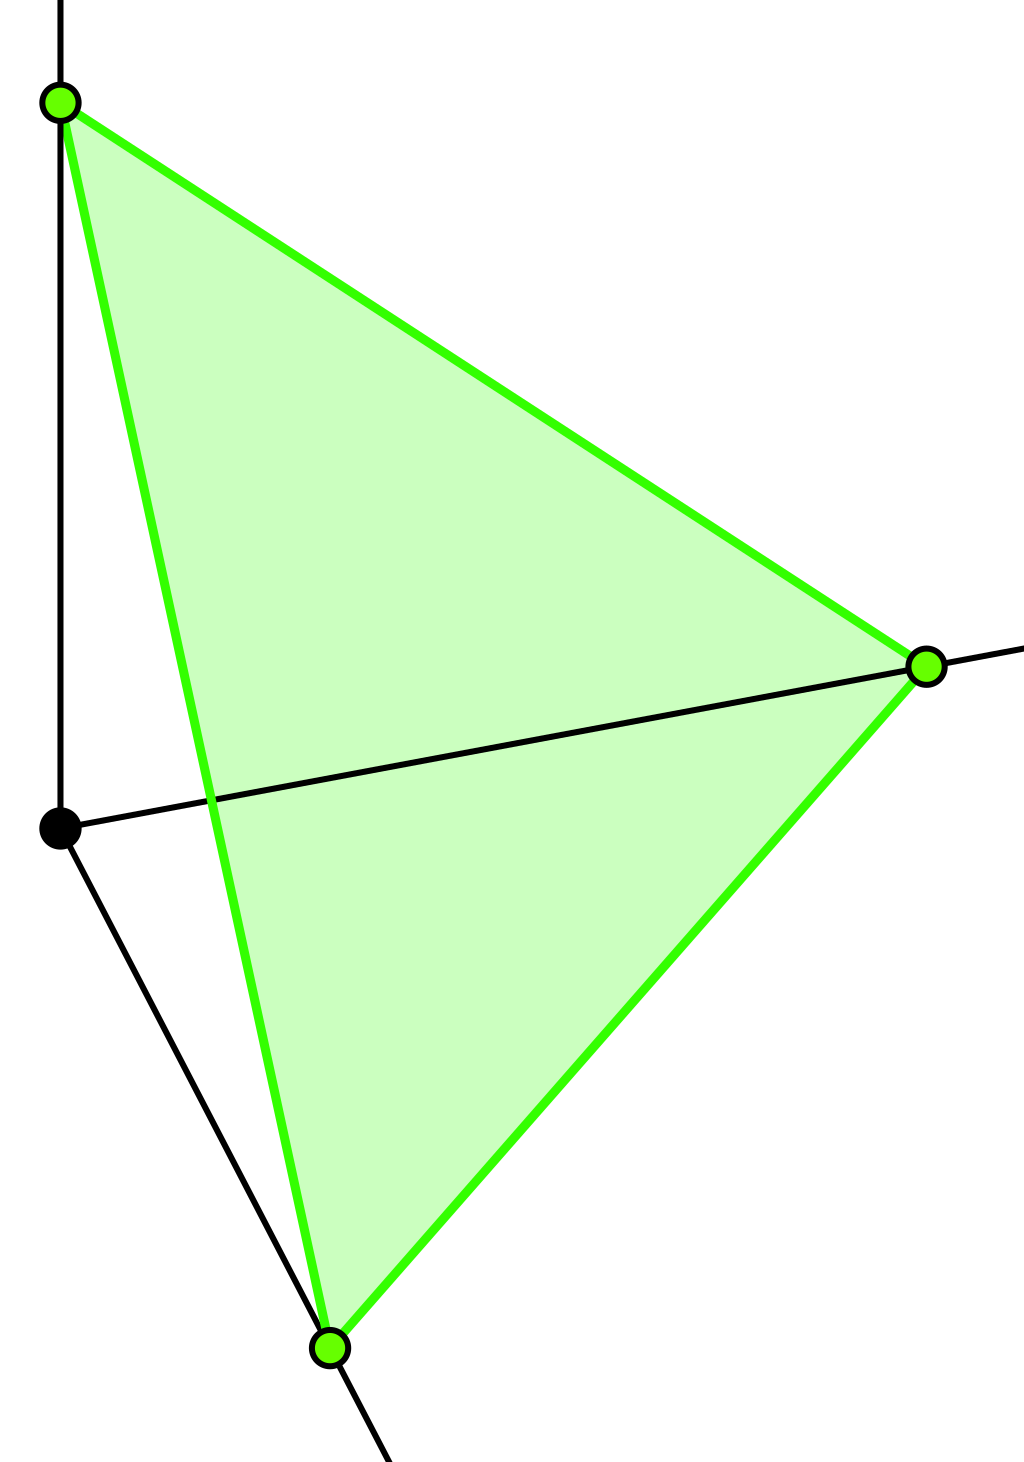
\includegraphics[scale=0.075]{standard-simplex-example.png}
    \end{figure}

    \begin{example}
        \phantom{a}
        \begin{enumerate}
            \item $\Delta^0$ is the point $1$ in $\bfR$
            \item $\Delta^1$ is the line segment joining $(0,1)$ and $(1,0)$ in $\bfR^2$.
            \item $\Delta^2$ is the equilateral triangle with vertices $(1,0,0)$, $(0,1,0)$, and $(0,0,1)$ in $\bfR^3$.
            \item $\Delta^3$ is the regular tetrahedron with vertices $(1,0,0,0)$, $(0,1,0,0)$, $(0,0,1,0)$, and $(0,0,0,1)$ in $\bfR^4$.
        \end{enumerate}
    \end{example}

    \begin{definition}
        If $X$ is a topological space, then the \textui{singular $n$-simplex in $X$} is a continuous map $\sigma : \Delta^n \rightarrow X$, where $\Delta^n$ is the standard $n$-simplex.
    \end{definition}

    \begin{definition}
        If $X$ is a topological space, define $S_n(X)$ to be the free abelian group whose basis is the set of all singular $n$-simplexes in $X$. The elements of $S_n(X)$ are called \textui{singular $n$-chains}.
    \end{definition}
\end{comment}
   
%%%%%%%%%%%%%%%%%%%%%%%%%%%%%%%%%%%%%%%%%%%%%%%%%%%%%%%%%%%%%%%%%%%%%%%%%%%%%%%%%%%%%%%%%%%%
%%%%%%%%%%%%%%%%%%%%%%%%%%%%%%%%%%%%%%%%%%%%%%%%%%%%%%%%%%%%%%%%%%%%%%%%%%%%%%%%%%%%%%%%%%%%
%%%%%%%%%%%%%%%%%%%%%%%%%%%%%%%%%%%%%%%%%%%%%%%%%%%%%%%%%%%%%%%%%%%%%%%%%%%%%%%%%%%%%%%%%%%%
%%%%%%%%%%%%%%%%%%%%%%%%%%%%%%%%%%%%%%%%%%%%%%%%%%%%%%%%%%%%%%%%%%%%%%%%%%%%%%%%%%%%%%%%%%%%
%%%%%%%%%%%%%%%%%%%%%%%%%%%%%%%%%%%%%%%%%%%%%%%%%%%%%%%%%%%%%%%%%%%%%%%%%%%%%%%%%%%%%%%%%%%%
\newpage
\section*{\centering Exercises}
    \addcontentsline{toc}{section}{\protect\numberline{}Exercises}
    \begin{exercise}
        Use parts (1) and (2) of Example~\ref{example:universal-properties} to show that if $\varphi:G \rightarrow H$ is a group homomorphism, then $G/\ker{\varphi} \cong \Image{\varphi}$.
    \end{exercise}
        {\color{red} \begin{proof}
            Since $\Image{\varphi}$ is a subgroup of $H$, the universal property of subgroups gives the correspondence $\varphi = \iota \circ \Phi$, where $\Phi : G \rightarrow \Image{\varphi}$ and $\iota: \Image{\varphi} \rightarrow H$. Now, since $\ker{\Phi}$ is a normal subgroup of $G$, the unversal property of quotient groups gives the correspondence $\Phi = \alpha \circ \pi$, where $\pi : G \rightarrow G/\ker{\Phi}$ and $\alpha: G/\ker{\Phi} \rightarrow \Image{\varphi}$. The following diagram commutes.

                \begin{center}
                    \begin{tikzcd}
                        &  & G/\ker{\Phi} \arrow[dd, "\mathlarger{\alpha}"]   \\
                        &  &                                     \\
                        G \arrow[rr, "\mathlarger{\Phi}"] \arrow[rruu, "\mathlarger{\pi}"] \arrow[rrdd, "\mathlarger{\varphi}"'] &  & \Image{\varphi} \arrow[dd, "\mathlarger{\iota}"] \\
                        &  &                                     \\
                        &  & H                                  
                    \end{tikzcd}
                \end{center}
            
            Claim: $\ker{\Phi} = \ker{\varphi}$. If $k \in \ker{\Phi}$, then $\Phi(k) = 0_{\Image{\varphi}} = 0_H$, hence $k \in \ker{\varphi}$. Conversely, if $k \in \ker{\varphi}$, then $k$ must get mapped to something inside the image of $\varphi$; i.e., $\varphi(k) = 0_H = 0_{\Image{\varphi}}$ implies $ k \in \ker{\Phi}$.

            Claim: $\alpha$ is an isomorphism. Note that $\Phi$ is clearly surjective, hence it must be the case that $\alpha$ is surjective. It remains to show that $\alpha$ is injective: this can be done by showing the map $\alpha : \G/\ker{\varphi} \rightarrow \Image{\varphi}$ has a trivial kernel. Let $g \in G$ be any element, note that $\alpha(g \ker{\varphi}) = \varphi(g)$ by our definition. Hence when $g \in \ker{\varphi}$, $\alpha(g \ker{\varphi}) = \alpha(\ker{\varphi}) = 0_{\Image{\varphi}}$ (the only element of $G/\ker{\varphi}$ which maps to $0_{\Image{\varphi}}$ is the identity). This establishes the proof that $G/\ker{\varphi} \cong \Image{\varphi}$\footnote{We can write $\varphi = \iota \circ \alpha \circ \pi$. In other words, \textit{every} momorphism takes the form of a quotient map, followed by an isomorphism, followed by an inclusion.}.
        \end{proof}}
    \begin{exercise}\label{ex:1-2}
        \phantom{a}
        \begin{enumerate}[label = (\roman*)]
            \item Prove, in every category $\mC$, that each object $A \in \mC$ has a unique identity morphism.
            \item If $f$ is an isomorphism in this category, prove that its inverse is unique.
        \end{enumerate}
    \end{exercise}
        {\color{red} \begin{proof}
            Let $f:A \rightarrow B$. Suppose $1_A,1_A' \in \Hom{(A,A)}$ such that $f1_A = f$ and $f1_A' = f$. Take $B=A$ and $f = 1_A'$, then $1_A' 1_A = 1_A '$. Now consider $g:B \rightarrow A$. Then  $1_A'g = g$. Take $B = A$ and $g = 1_A$, then $1_A'1_A = 1_A$. Together, this gives $1_A' = 1_A' 1_A = 1_A$. Hence the identity morphism is unique.

            Let $f:A \rightarrow B$ be an isomorphism. Suppose $g,g' : B \rightarrow A$ are inverses of $f$. Then
            $g = 1_A g = (g'f)g = g'(fg) = g'1_B = g'$. Hence inverses are unique.
        \end{proof}}

    \begin{exercise}\label{ex:1-3}
        If $T:\mA \rightarrow \mB$ is a functor, define $T^\text{op}: \mA^\text{op} \rightarrow \mB$ by $T^\text{op}(A) = T(A)$ for all $A \in \obj{(\mA)}$ and $T^\text{op}(f^\text{op}) = T(f)$ for all morphisms $f$ in $\mA$. Prove that $T^\text{op}$ is a functor having variance opposite to the variance of $T$.
    \end{exercise}
    
    \begin{exercise}
        \phantom{a}
        \begin{enumerate}[label = (\roman*)]
            \item If $X$ is a set, define $FX$ to be the free group having basis $X$, that is, the elements of $FX$ are reduced words on the alphabet $X$ and multiplication is juxtaposition followed by cancellation. If $\varphi:X \rightarrow Y$ is a function, prove that there is a unique homomorphism $F\varphi:FX \rightarrow FY$ such that $(F\varphi)\mid X = \varphi$.
            \item Prove that $F:\cSets \rightarrow \cGroups$ is a functor ($F$ is called the \textui{free functor}).
        \end{enumerate}
    \end{exercise}

    \begin{exercise}
        \phantom{a}
        \begin{enumerate}[label = (\roman*)]
            \item Define $\mC$ to have objects all ordered pairs $(G,H)$, where $G$ is a group and $H$ is a normal subgroup of $G$, and to have morphisms $\varphi_*:(G,H) \rightarrow (G_1,H_1)$, where $\varphi:G \rightarrow G_1$ is a homomorphism with $\varphi(H) \subseteq H_1$. Prove that $\mC$ is a category if composition in $\mC$ is defined to be ordinary composition.
            \item Construct a functor $Q: \mC \rightarrow \cGroups$ with $Q(G,H) = G/H$.
            \item Prove that there is a functor $\cGroups \rightarrow \cAb$ taking each group $G$ to $G/G'$, where $G'$ is its commutator subgroup.
        \end{enumerate}
    \end{exercise}

    \begin{exercise}
        Let $R$ be a ring. An (additive) abelian group $M$ is an \textui{almost left $R$-module} if there is a function $R \times M \rightarrow M$ which satisfies all of the left $R$-module axioms except for Axiom (4): we do not assume that $1m = m$ for all $m \in M$. Prove that if $M$ is an almost left $R$-module then $M = M_1 \oplus M_0$, where $M_1 = \{m \in M:1m = 1\}$ and $M_0 = \{m \in M: rm = 0 \hspace{4pt} \text{for all $r \in R$}\}$ are subgroups of $M$ that are almost left $R$-modules (in fact, $M_1$ is a left $R$-module).
    \end{exercise}
        {\color{red}\begin{proof}   
            
        \end{proof}}

    \begin{exercise}
        Prove that every right $R$-module is a left $R^\text{op}$-module and vice versa.
    \end{exercise}

    \begin{exercise}\label{exer:1-8}
        Let $M$ be a left $R$-module.
        \begin{enumerate}[label = (\roman*)]
            \item Prove that $\Hom_R{(M,M)}$ is a ring with $1$ under pointwise addition and composition as multiplication.
            \item The ring $\Hom_R{(M,M)}$ is called the \textui{endomorphism ring of $M$} and is denoted $\End_R(M)$. Elements of $\End_R(M)$ are called \textui{endomorphisms}. Prove that $M$ is a left $\End_R(M)$-module.
            \item If a ring $R$ is regarded as a left $R$-module, prove that $\End_R(R) \cong R^\text{op}$ as rings.
        \end{enumerate}
    \end{exercise}
        {\color{red} \begin{proof}
            The details of $\Hom_R{(M,M)}$ being an abelian group are left out \textemdash associativity and commutativity are shown easily, the identity is the zero map $0_{MM}$ and inverses follow from this. Let $\varphi,\psi, \gamma \in \Hom_R{(M,M)}$. Note that function composition is automatically associative. "$1$" in this case is the identity morphism: $(\varphi \circ \id_{M})(m) = \varphi(\id_M(m)) = \varphi(m)$ and $(\id_M \circ \varphi)(m) = \id_M(\varphi(m)) = \varphi(m)$. Function composition distributes over pointwise addition as follows:
                \begin{equation*}
                \begin{split}
                    (\varphi \circ (\psi + \gamma))(m)
                    & = \varphi((\psi + \gamma)(m)) \\
                    & = \varphi(\psi(m) + \gamma(m)) \\
                    & = \varphi(\psi(m)) + \varphi(\psi(m))\\
                    & = (\varphi \circ \psi)(m) + (\varphi \circ \gamma)(m)\\
                    & = ((\varphi \circ \psi) + (\varphi \circ \gamma))(m).
                \end{split}
                \end{equation*}
            Distribution from the right follows similary, hence $\Hom_R{(M,M)}$ is a unital ring.


        \end{proof}}

    \chapter{Module Theory}\label{chapter:module-theory}

\pagenumbering{arabic}

\section{Basic Definitions and Examples}\label{sec:basic-defs-examples}
    \begin{definition}\label{def:module-axioms}
        Let $R$ be a ring (not necessarily commutative nor with $1$). A \textui{left $R$-module} or a \textui{left module over $R$} is a set $M$ together with:
        \begin{enumerate}[label = (\arabic*)]
            \item a binary operation $+$ on $M$ under which $M$ is an abelian group, and
            \item an action of $R$ on $M$ (that is, a map $R \times M \rightarrow M$) denoted by $rm$ for all $r \in R$ and for all $m \in M$ which satisfies:
            \begin{enumerate}[label = (\alph*)]
                \item $(r+s)m = rm + rs$,\quad for all $r,s \in R$, $m \in M$
                \item $(rs)m = r(sm)$,\quad for all $r,s \in R$, $m \in M$
                \item $r(m+n) = rm + rn$,\quad for all $r \in R$, $m,n \in M$.
            \end{enumerate}
            If the ring $R$ has a $1$ we impose the additional axiom:
            \begin{enumerate}[label = (\alph*)]
                \addtocounter{enumii}{3}
                \item $1m = m$,\quad for all $m \in M$.
            \end{enumerate}
        \end{enumerate}
    \end{definition}

    \begin{note}
        Modules over a field $F$ and vector spaces over $F$ are the same.
    \end{note}

    \begin{definition}\label{def:submodule}
        Let $R$ be a ring and let $M$ be an $R$-module. An \textui{$R$-submodule of $M$} is a subgroup $N$ of $M$ which is closed under the action of ring elements; i.e., $rn \in N$ for all $r \in R$, $n \in N$.
    \end{definition}

    \begin{example}
        \phantom{a}
        \begin{enumerate}[label = (\arabic*)]
            \item Let $R$ be any ring. Then $M = R$ is a left $R$-module. The ring action is just normal multiplication in the ring $R$. When $R$ is a left module over itself, the submodules of $R$ are the left ideals of $R$. IF $R$ is not commutative its left and right module structure over itself might be different
            \item Let $R = F$ be a field. Note that every vector space over $F$ is an $F$-module and vice versa. Define
                \begin{equation*}
                \begin{split}
                F^n = \{(a_1,a_2,...,a_n) \mid a_i \in F, n \in \bfZ^{+}\}
                \end{split}
                \end{equation*}
            as \textui{affine $n$-space over $F$}. We can make $F^n$ into a vector space by defining addition and scalar multiplication componentwise. When $F = \bfR$ we have the familiar Euclidean $n$-space.
            \item If $M$ is an $R$-module and $S$ is a subring of $R$ with $1_R = 1_S$, then $M$ is an $S$-module as well. For example, the field $\bfR$ is an $\bfR$-module, a $\bfQ$-module, and a $\bfZ$-module.
        \end{enumerate}
    \end{example}

    \begin{example}[$\bfZ$-Modules]
        Let $R = \bfZ$, let $A$ be any abelian group and write the operation of $A$ as $+$. Make $A$ into a $\bfZ$-module as follows: for any $n \in \bfZ$ and $a \in A$ define
        \begin{equation*}
        na = 
        \begin{cases} 
        a + a + ... + a \text{\quad ($n$ times)} & \quad \text{if}\hskip0.4em\relax n>0 \\
        0 & \quad \text{if}\hskip0.4em\relax n=0 \\
        -a - a - ... - a \text{\quad ($n$ times)} & \quad \text{if}\hskip0.4em\relax n<0\hskip0.4em\relax, 
        \end{cases}
        \end{equation*}
        where $0$ is the identity of the additive abelian group $A$. This definition of $\bfZ$ acting on $A$ makes $A$ into a $\bfZ$-module, and furthermore the module axioms show that this is the only action of $\bfZ$ on $A$. Thus every abelian group is a $\bfZ$-module and vice versa. Furthermore $\bfZ$-submodules are the same as subgroups.
    \end{example}

    \begin{proposition}[The Submodule Criterion]\label{prop:submodule-criterion}
        Let $R$ be a ring and let $M$ be an $R$-module. A subset $N$ of $M$ is a submodule of $M$ if and only if $N \neq \emptyset$ and $x+ry \in N$ for all $r \in R$ and $x,y \in N$.
        \begin{proof}
            If $N$ is a submodule, then $0 \in N$  so $N \neq \emptyset$. Also $N$ is closed under addition and is sent to itself under the action of elements in $R$\footnote{This satisfies axioms $(1)$ and $(2)$ from Definition~\ref{def:module-axioms}}.  

            Conversely, suppose $N \neq \emptyset$ and $x+ry \in N$ for all $r \in R$ and $x,y \in N$. Let $r = -1$, then $x-y \in N$; i.e., $N$ is a subgroup of $M$. This also gives that $0 \in N$. Let $x = 0$, then $ry \in N$; i.e., $N$ is sent to itself under the action of $R$. This establishes the proposition.
        \end{proof}
    \end{proposition}

    \begin{definition}\label{def:r-algebra}
        Let $R$ be a commutative ring with identity. An \textui{$R$-algebra} is a ring $A$ with identity together with a ring homomorphism $f: R \rightarrow A$ mapping $1_R$ to $1_A$ such that the subring $f(R)$ of $A$ is contained in the center of $A$. That is, $f(R) \subseteq \text{Z}(A)$.
    \end{definition}

    \begin{definition}\label{def:r-algeba-homomorphism}
        If $A$ and $B$ are two $R$-algebras, an \textui{$R$-algebra homomorphism} (or isomorphism) is a ring homomorphism (isomorphism, respectively) $\varphi:A \rightarrow B$ mapping $1_A$ to $1_B$ such that $\varphi(ra) = r\varphi(a)$ for all $r \in R$ and $a \in A$.
    \end{definition}

    \begin{definition}\label{def:torsions-and-annihilators}
        Let $R$ be a ring and $M$ and $R$-module. 
        \begin{enumerate}[label=(\arabic*)]
            \item An element $m$ of the $R$-module $M$ is called a \textui{torsion element} if $rm=0$ for some nonzero element $r \in R$. The set of torsion elements is denoted
                \begin{equation*}
                \begin{split}
                    \text{Tor}(M)=\{m \in M \mid rm=0\quad \text{for some nonzero $r \in R$}\}.
                \end{split}
                \end{equation*}
            \item If $N$ is a submodule of $M$ the \textui{annihilator of $N$ in $R$} is defined to be
                \begin{equation*}
                \begin{split}
                    \text{Ann}_R(N) = \{r \in R \mid rn = 0 \quad \text{for all $n \in N$}\}.
                \end{split}
                \end{equation*}
            \item If $I$ is a right ideal of $R$, the \textui{annihilator of $I$ in $M$} is defined to be
                \begin{equation*}
                \begin{split}
                    \text{Ann}_M(I) = \{m \in M \mid am = 0 \quad \text{for all $a \in I$}\}.
                \end{split}
                \end{equation*}
        \end{enumerate}
    \end{definition}

\section{Quotient Modules and Module Homomorphisms}\label{sec:quotient-homoms}
    \begin{definition}\label{def:module-homomorphism}
        Let $R$ be a ring and let $M$ and $N$ be $R$-modules.
        \begin{enumerate}[label=(\arabic*)]
            \item A map $\varphi:M \rightarrow N$ is an \textui{$R$-module homomorphism} if it respects the $R$-module structures of $M$ and $N$; i.e.,
            \begin{enumerate}[label=(\alph*)]
                \item $\varphi(x+y) = \varphi(x) + \varphi(y)$ for all $x,y \in M$ and
                \item $\varphi(rx) = r\varphi(x)$ for all $r \in R$, $x \in M$.
            \end{enumerate}
            \item An $R$-module homomorphism is an \textui{isomorphism} (of $R$-modules) if it is both injective and surjective. The modules $M$ and $N$ are said to be \textui{isomorphic}, denoted $M \cong N$, if there is some $R$-module isomorphism $\varphi:M \rightarrow N$.
            \item If $\varphi:M\rightarrow N$ is an $R$-module homomorphism, let $\ker{\varphi} = \{m \in M \mid \varphi(m) = 0\}$ and let $\Image{\varphi}=\{n \in N \mid n = \varphi(m)\quad\text{for some $m \in M$}\}$.
            \item Let $M$ and $N$ be $R$-modules and define $\Hom_R{(M,N)}$ to be the set of all $R$-module homomorphisms from $M$ into $N$.
        \end{enumerate}
    \end{definition}

    \begin{note}
        Any $R$-module homomorphism is also a homomorphism of the additive groups, but not every group homomorphism need be a module homomorphism (condition (b) may not be satisfied).
    \end{note}

    \begin{example}
        \phantom{a}
        \begin{enumerate}[label=(\arabic*)]
            \item If $R$ is a ring and $M=R$ is a module over itself, then $R$-module homomorphisms need not be ring homomorphisms and vice versa. For example, when $R = \bfZ$ the $\bfZ$-module homomorphism $x \mapsto 2x$ is not a ring homomorphism ($1$ does not get mapped to $1$).
            \item When $R$ is a field, $R$-module homomorphisms are called \textui{linear transformations}.
            \item $\bfZ$-module homomorphisms are the same as abelian group homomorphisms; i.e., from Definition~\ref{def:module-homomorphism} condition (b) is implied by condition (a). For example, $\varphi(2x) = \varphi(x + x) = \varphi(x) + \varphi(x) = 2\varphi(x)$.
            \item Let $R$ be a ring, let $I$ be a two sided ideal of $R$ and suppose $M$ and $N$ are $R$-modules annihilated by $I$ (i.e., $am=0$ and $an=0$ for all $a \in I$, $m \in M$, and $n \in N$). Any $R$-module homomorphism from $N$ to $M$ is then automatically a homomorphism of $(R/I)$-modules.
        \end{enumerate}
    \end{example}

    \begin{proposition}\label{prop:properties-of-hom}
        Let $M,N$, and $L$ be $R$-modules.
        \begin{enumerate}[label = (\arabic*)]
            \item A map $\varphi:M \rightarrow N$ is an $R$-module homomorphism if and only if $\varphi(rx+y) = r\varphi(x) + \varphi(y)$ for all $x,y \in M$ and all $r \in R$.
            \item Let $\varphi, \psi$ be elements of $\Hom_R{(M,N)}$ Define $\varphi + \psi$ by 
                \begin{equation*}
                \begin{split}
                    (\varphi+\psi)(m) = \varphi(m) + \psi(m) \quad \text{for all $m \in M$}.
                \end{split}
                \end{equation*}
            Then $\varphi + \psi \in \Hom_R{(M,N)}$ and with this operation $\Hom_R{(M,N)}$ is an abelian group. If $R$ is a commutative ring then for $r \in R$ define $r\varphi$ by:
                \begin{equation*}
                \begin{split}
                    (r\varphi)(m) = r\varphi(m) \quad \text{for all $m \in M$}.
                \end{split}
                \end{equation*}
            Then $r\varphi \in \Hom_R{(M,N)}$ and with this action of the commutative ring $R$ the abelian group $\Hom_R{(M,N)}$ is an $R$-module.
            \item If $\varphi \in \Hom_R{(L,M)}$ and $\psi \in \Hom_R{(M,N)}$ then $\psi \circ \varphi \in \Hom_R{(L,N)}$.
            \item With addition as above and multiplication defined as function composition, $\Hom_R{(M,M)}$ is a ring with $1$. When $R$ is commutative $\Hom_R{(M,M)}$ is an $R$-algebra.
        \end{enumerate}
    \end{proposition}
    \begin{proof}
        (1) Certainly if $\varphi$ is an $R$-module homomorphism then $\varphi(rx+y) = r\varphi(x) + \varphi(y)$. Conversely, if $\varphi(rx+y) = r\varphi(x) + \varphi(y)$, take $r = 1$ to see that $\varphi$ is additive and take $y = 0$ to see that $\varphi$ commutes with the action of $R$ on $M$.\footnote{We say $\varphi$ is \textui{homogeneous} in this case.}

        (2) It is straightforward to check that all the abelian group and $R$-module axioms hold with these definitions. For example $r\varphi$ satisfies (b) from Definition~\ref{def:module-axioms} as follows:
            \begin{equation*}
            \begin{split}
                (r_1\varphi)(r_2 m)
                & = r_1 \varphi(r_2 m) \\
                & = r_1 r_2 \varphi(m) \\
                & = r_2 r_1 \varphi(m) \\
                & = r_2 (r_1\varphi)(m).
            \end{split}
            \end{equation*}

        (3) Let $\varphi$ and $\psi$ be as given and let $r \in R$ and $x,y \in L$. Then:
            \begin{equation*}
            \begin{split}
                (\psi \circ \varphi)(rx+y)
                & = \psi(\varphi(rx+y)) \\
                & = \psi(r\varphi(x) + \varphi(y)) \\
                & = r\psi(\varphi(x)) + \psi(\varphi(y)) \\
                & = r(\psi \circ \varphi)(x) + (\psi \circ \varphi)(y).
            \end{split}
            \end{equation*}
        So, by (1) from this proposition, $\psi \circ \varphi$ is an $R$-module homomorphism.

        (4) Note that since the domain and codomain of the elements of $\Hom_R{(M,M)}$ are the same, function composition is defined. By (3) from this proposition, it is a binary operation on $\Hom_R{(M,M)}$. As usual function composition is associative. The remaining ring axioms are straight foward to check. The identity function, $I$, ($I(x) = x$ for all $x \in M$) is seen to be the multiplicative identity of $\Hom_R{(M,M)}$. If $R$ is commutative, then (2) from this proposition shows that the ring $\Hom_R{(M,M)}$ is a left $R$-module and defining $\varphi r = r\varphi$ for all $\varphi \in \Hom_R{(M,M)}$ and $r \in R$ makes $\Hom_R{(M,M)}$ into an $R$-algebra.
    \end{proof}

    \begin{definition}\label{def:endomorphism-ring}
        The ring $\Hom_R{(M,M)}$ is called the \textui{endomorphism ring of $M$} and is denoted $\End_R(M)$. Elements of $\End_R(M)$ are called \textui{endomorphisms}.
    \end{definition}

    \begin{note}
        Let $H$ be a subgroup of $G$. If $G$ is abelian then $H$ is normal. This is relevant for the following proposition.
    \end{note}

    \begin{proposition}
        Let $R$ be a ring, let $M$ be an $R$-module and let $N$ be a submodule of $M$. The (additive, abelian) quotient group $M/N$ can be made into an $R$-module by defining an action of elements of $R$ by
            \begin{equation*}
            \begin{split}
                r(x+N) = rx + N \quad \text{for all $r \in R$, $x + N \in M/N$}.
            \end{split}
            \end{equation*}
        The natural projection map $\pi:M \rightarrow M/N$ defined by $\pi(x) = x +N$ is an $R$-module homomorphism with kernel $N$.
    \end{proposition}
    \begin{proof}
        Since $M$ is an abelian group under $+$ the quotient group $M/N$ is defined and is an abelian group. We must show that the action of the ring element $r$ on the coset $x + N$ is well defined. Suppose $x + N = y+ N$; i.e., $x-y \in N$. Since $N$ is a (left) $R$-module, $r(x-y) \in N$. Thus $rx-ry \in N$; i.e., $rx + N = ry + N$.

        Since the operations in $M/N$ are "compatible" with those of $M$, the axioms for an $R$-module are easily checked. Likewise, the natural projection map $\pi$ described as above is, in particular, the natural projection of the abelian group $M$ onto the abelian group $M/N$ hence is a group homomorphism with kernel $N$. The kernel of any module homomorphism is the same as its kernel when viewed as a homomorphism of the abelian group structures. It remains to show that $\pi$ is a module homomorphism \textemdash which it is: $\pi(rm) = rm + N = r(m+N) = r\pi(m)$.
    \end{proof}

    \begin{definition}\label{def:module-sum}
        Let $A,B$ be submodules of the $R$-module $M$. The \textui{sum} of $A$ and $B$ is the set $A+B = \{a+b \mid a \in A, b\in B\}$.
    \end{definition}

    \begin{definition}[Isomorphism Theorems]\label{def:module-iso-thms}
        \phantom{a}
        \begin{enumerate}[label = (\arabic*)]
            \item 
            \item
            \item 
            \item
        \end{enumerate}
    \end{definition}

\section{Generation of Modules, Direct Sums, and Free Modules}
    \begin{definition}\label{def:-properties-module-sums}
        Let $M$ be an $R$-module and let $N_1,...,N_n$ be submodules of $M$.
        \begin{enumerate}[label = (\arabic*)]
            \item The \textui{sum} of $N_1,...,N_n$ is the set of all finite sums of elements from the sets $N_i$: $\{a_1 + a_2 + ... + a_n \mid a_i \in N_i \hskip0.4em\relax \text{for all }i\}$. Denote this sum by $N_1 + N_2 + ... + N_n$.
            \item For any subset $A$ of $M$ let
            \begin{equation*}
            \begin{split}
                RA = \{r_1 a_1 + r_2 a_2 + ... + r_m a_m \mid r_1,...,r_m \in R,\hskip0.4em\relax a_1,...,a_m \in A,\hskip0.4em\relax m \in \bfZ^{+}\}
            \end{split}
            \end{equation*}
            (where by convention $RA = \{0\}$ if $A = \emptyset$). If $A$ is the finite set $\{a_1,a_2,...,a_n\}$ we shall write $Ra_1 + Ra_2 + ... + Ra_n$ for $RA$. Call $RA$ the \textui{submodule of $M$ generated by $A$}. If $N$ is a submodule of $M$ (possibly $N = M$) and $N=RA$ for some subset $A$ of $M$, we call $A$ a \textui{set of generators} or \textui{generating set} for $N$, and we say $N$ is \textui{generated} by $A$.
            \item A submodule $N$ of $M$ (possibly $N=M$) is \textui{finitely generated} if there is some finite subset $A$ of $M$ such that $N = RA$, that is, if $N$ is generated by some finite subset.
            \item A submodule $N$ of $M$ (possibly $N=M$) is \textui{cyclic} if there exists an element $a \in M$ such that $N = Ra$, that is, if $N$ is generated by one element:
            \begin{equation*}
            \begin{split}
                N = RA = \{ra \mid r \in R\}.
            \end{split}
            \end{equation*}
        \end{enumerate}
    \end{definition}

    \begin{definition}\label{def:external-direct-sum}
        Let $M_1,...,M_k$ be a collection of $R$-modules. The collection of $k$-tuples $(m_1,...,m_k)$ where $m_i \in M_i$ with addition and action of $R$ defined componentwise is called the \textui{direct product} of $M_1,...,M_k$, denoted $M_1 \times ... \times M_k$. The direct product of $M_1,...,M_k$ is also referred to as the (external) \textui{direct sum} of $M_1,...,M_k$ and is denoted $M_1 \oplus ... \oplus M_k$.
    \end{definition}

    \begin{proposition}\label{prop:properties-of-direct-prods}
        Let $N_1,N_2,...,N_k$ be submodules of the $R$-module $M$. Then the following are equivalent:
        \begin{enumerate}[label = (\arabic*)]
            \item The map $\pi:N_1 \times N_2 \times ... \times N_k \rightarrow N_1 + N_2 + ... + N_k$ defined by 
                \begin{equation*}
                \begin{split}
                    \pi((a_1,a_2,...,a_k)) = a_1 + a_2 + ... +a_k
                \end{split}
                \end{equation*}
            is an isomorphism (of $R$-modules): $N_1 \times N_2 \times ... \times N_k \cong N_1 + N_2 + ... + N_k$.
            \item $N_j \cap (N_1 + N_2 + ... + N_{j-1} + N_{j+1} + ... + N_k) = 0$ for all $j \in \{1,2,...,k\}$.
            \item Every $x \in N_1 + N_2 + ... + N_k$ can be written uniquely in the form $a_1 + a_2 + ... + a_k$ with $a_i \in N_i$.
        \end{enumerate}
    \end{proposition}
    \begin{proof}
        To prove that (1) implies (2), suppose for some $j$ (2) fails to hold and let $a_j \in N_j \cap (N_1 + N_2 + ... + N_{j-1} + N_{j+1} + ... + N_k)$ with $a_j \neq 0$. Then $a_j \in N_j$ and $a_j \in N_1 + N_2 + ... + N_{j-1} + N_{j+1} + ... + N_k$, hence $a_j = a_1 + a_2 + ... + a_{j-1} + a_{j+1} + ... + a_k$ for some $a_i \in N_i$. Subtracting $a_j$ from both sides gives $0 = a_1 + a_2 + ... + a_{j-1} -a_j + a_{j+1} + ... + a_k$, which is equivalent to $\pi(0) = (a_1,a_2,...,a_{j-1},-a_j,a_{j+1},...,a_k)$. Note that this would be a nonzero element of $\ker{\pi}$, which gives a contradiction.

        Assume now that (2) holds. If for some module elements $a_i , b_i \in N_i$ we have: $$a_1+a_2+...+a_k = b_1+b_2+...+b_k$$ then for each $j$ we have: $$a_j - b_j = (b_1 - a_1)+ (b_2 - a_2)+ ... + (b_{j-1} - a_{j-1}) + (b_{j+1} - a_{j+1}) + ... + (b_k - a_k).$$ The left belongs to $N_j$ and the right side belongs to $(N_1 + N_2 + ... + N_{j-1} + N_{j+1} + ... + N_k)$, hence $a_j - b_j \in N_j \cap (N_1 + N_2 + ... + N_{j-1} + N_{j+1} + ... + N_k)$. It must be the case then that $a_j - b_j = 0$; i.e., $a_j = b_j$ for all $j$. Thus (2) implies (3).

        Finally, to see that (3) implies (1), observe first that the map $\pi$ is clearly a surjective $R$-module homomorphism. Then $(3)$ simply implies $\pi$ is injective, hence is an isomorphism, completing the proof.
    \end{proof}

    \begin{definition}\label{def:internal-direct-sum}
        If an $R$-module $M$ is the sum of submodules $N_1, N_2, ... , N_k$ of $M$ satisfying the conditions of the proposition above, then $M$ is said to be the (internal) \textui{direct sum} of $N_1, N_2, ..., N_k$, written:
            \begin{equation*}
            \begin{split}
                M = N_1 \oplus N_2 \oplus ... \oplus N_k.
            \end{split}
            \end{equation*}
    \end{definition}

    \begin{note}
        Part (1) of Proposition~\ref{prop:properties-of-direct-prods} is the statement that the internal direct sum of $N_1,N_2,...,N_k$ is isomorphic to their external direct sum (from Definition~\ref{def:external-direct-sum}), which is the reason we identify them and use the same notation for both.
    \end{note}

    \begin{definition}\label{def:free-modules}
        An $R$-module $F$ is said to be \textui{free} on the subset $A$ of $F$ if for every nonzero element $x$ of $F$, there exist unique nonzero elements $r_1,r_2,...,r_n$ of $R$ and unique $a_1,a_2,...,a_n$ in A such that $x = r_1 a_1 + r_2 a_2 + .... + r_n a_n$, for some $n \in \bfZ^{+}$. In this situation we say $A$ is a \textui{basis} or \textui{set of free generators} for $F$. If $R$ is a commutative ring the cardinality of $A$ is called the \textui{rank} of $F$.
    \end{definition}

    \begin{note}
        To avoid confusion, we reiterate Definition~\ref{def:-properties-module-sums} and Definition~\ref{def:free-modules} as follows: An $R$-module $M$ is called:
        \begin{itemize}
            \item \textui{free} if $M \cong R^n = \bigoplus_{i=1}^{n} R$. In other words, the map $\phi:R^n \rightarrow M$ is an $R$-module isomorphism. $n$ is called the \textui{rank} of $M$ and it can be infinite.
            \item \textui{finitely generated} if $M$ has a finite generating set. In other words, the map $\phi:R^n \rightarrow M$ is only surjective.
        \end{itemize}
        The difference boils down to whether $\ker{\phi}=0$ or not. Furthermore, in the case of a direct sum between two modules, the module elements will be unique, whereas in the case of free modules the module elements and ring elements must be unique.
    \end{note}
    
    \begin{theorem}\label{thm:universal-property}
        For any set $A$ there is a free $R$-module $F(A)$ on the set $A$ where $F(A)$ satisfies the following \textit{universal property}: if $M$ is any $R$-module and $\varphi:A \rightarrow M$ is any map of sets, then there is a unique $R$-module homomorphism $\phi:F(A) \rightarrow M$ such that $\phi(a) = \varphi(a)$ for all $a \in A$, that is, the following diagram commutes:
        \begin{center}
                \begin{tikzcd}
                A \arrow[rr, "\text{inclusion}"] \arrow[rrdd, "\mathlarger{\varphi}"'] &  & F(A) \arrow[dd, "\mathlarger{\phi}"] \\
                                                          &  &                         \\
                                                          &  & M                      
            \end{tikzcd}
        \end{center}
    \end{theorem}
    \begin{proof}
        Let $F(A)=\{0\}$ if $A = \emptyset$. If $A$ is nonempty let $F(A)$ be the collection of all set functions $f:A \rightarrow R$ such that $f(a) = 0$ for all but finitely many $a \in A$. Make $F(A)$ into an $R$-module by pointwise addition of functions and pointwise multiplication of a ring element times a function. It is an easy matter to check that all $R$-module axioms hold. Identify $A$ as a subset of $F(A)$ by $a \mapsto f_a$, where $f_a$ is the function which is 1 at $a$ and zero elsewhere. We can, in this way, think of $F(A)$ as all finite $R$-linear combinations of elements of $A$ by identifying each function $f$ with the sum $r_1 a_1 + r_2 a_2 + ... + r_n a_n$, where $f$ takes on the value $r_i$ at $a_i$ and is zero at all other elements of $A$. To establish the universal property of $F(A)$ suppose $\varphi:A \rightarrow M$ is a map of the set $A$ into the $R$-module $M$. Define $\phi:F(A) \rightarrow M$ by
            \begin{equation*}
            \begin{split}
                \phi:\sum_{i=1}^{n}r_i a_i \mapsto \sum_{i=1}^{n}r_i \varphi(a_i).
            \end{split}
            \end{equation*}
        By the uniqueness of the expression for the elements of $F(A)$ as linear combinations of the $a_i$ we see easily that $\phi$ is a well defined $R$-module homomorphism. By definition, the restriction of $\phi$ to $A$ equals $\varphi$. Finally, since $F(A)$ is generated by $A$, once we know the values of an $R$-module homomorphism on $A$ its values on every element of $F(A)$ are uniquely determined, so $\phi$ is the unique extension of $\varphi$ to all of $F(A)$.
    \end{proof}

    \begin{corollary}
        \phantom{a}
        \begin{enumerate}[label=(\arabic*)]
            \item If $F_1$ and $F_2$ are free modules on the same set $A$, there is a unique isomorphism between $F_1$ and $F_2$ which is the identity map on $A$.
            \item If $F$ is any free $R$-module with basis $A$, then $F \cong F(A)$. In particular, $F$ enjoys the same universal property with respect to $A$ as $F(A)$ does in Theorem~\ref{thm:universal-property}.
        \end{enumerate}
    \end{corollary}
    \begin{proof}
        Exercise.
    \end{proof}

\section{Tensor Products of Modules}
    \begin{definition}\label{def:biadditive-bilinear}
        Let $R$ be a ring, let $A$ be a right $R$-module, let $B$ be a left $R$-module, and let $G$ be an (additive) abelian group. A function $f:A\times B \rightarrow G$ is called \textui{$R$-biadditive} if, for all $a,a' \in A$, $b,b' \in B$, and $r \in R$ we have
            \begin{enumerate}[label=(\arabic*)]
                \item $f(a+a',b) = f(a,b) + f(a',b),$
                \item $f(a,b+b') = f(a,b) + f(a,b'),$
                \item $f(ar,b) = f(a,rb).$
            \end{enumerate}
        If $R$ is commutative and $A,B$, and $M$ are $R$-modules, then a function $f:A\times B \rightarrow M$ is called \textui{$R$-bilinear} if $f$ is $R$-biadditive and also 
            \begin{enumerate}[label=(\arabic*)]
                \addtocounter{enumi}{3}
                \item $f(ar,b) = f(a,rb) = rf(a,b)$.
            \end{enumerate}
    \end{definition}

    \begin{example}
        \phantom{a}
        \begin{enumerate}[label = (\arabic*)]
            \item If $R$ is a ring, then its multiplication $\mu:R \times R \rightarrow R$ is $R$-biadditive; the first two axioms from Definition~\ref{def:biadditive-bilinear} are the right and left distributive laws, while the third axiom is associativity:
                \begin{equation*}
                \begin{split}
                    \mu(ar,b)=(ar)b=a(rb)=\mu(a,rb).
                \end{split}
                \end{equation*}
            If $R$ is a commutative ring, then $\mu$ is $R$-bilinear, for $(ar)b=a(rb)=r(ab)$.

            \item If we regard a left $R$-module $M$ as its underlying abelian group, then the scalar multiplication $\sigma: R \times M \rightarrow M$ is $\bfZ$-bilinear.

            \item Recall from Proposition~\ref{prop:properties-of-hom} that $\Hom_R{(M,N)}$ is an $R$-module if $R$ is commutative and we define $(r\varphi)(m)=r(\varphi(m))$ for all $m \in M$. With this definition we can see that \textui{evaluation} $e:M \times \Hom_R{(M,N)} \rightarrow N$ given by $(m,\varphi) \mapsto \varphi(m)$ is $R$-bilinear.
        \end{enumerate}
    \end{example}

    \begin{definition}\label{def:tensor-product}
        Given a ring $R$, a left $R$-module $A$, and a right $R$-module $B$, then their \textui{tensor product} is an abelian group $A \otimes_R B$ and an $R$-biadditive function
            \begin{equation*}
            \begin{split}
                h:A \times B \rightarrow A \otimes_R B
            \end{split}
            \end{equation*}
        such that, for every abelian group $G$ and every $R$-biadditive function $f:A \times B \rightarrow G$, there exists a unique $\bfZ$-homomorphisms $\tilde{f}:A \otimes_R B \rightarrow G$ making the following diagram commute:
            \begin{center}
            \begin{tikzcd}
                A \times B \arrow[rd, "\mathlarger{f}"'] \arrow[rr, "\mathlarger{h}"] &   & A \otimes_R B \arrow[ld, "\mathlarger{\tilde{f}}", dashed] \\
                                            & G &                                              
            \end{tikzcd}
            \end{center}
    \end{definition}

    \begin{definition}\label{def:bimodules}
        Let $R$ and $S$ be rings and let $M$ be an abelian group. Then $M$ is an \textui{$(R,S)$-bimodule}, denoted by $\phantom{.}_R M_S$, if $M$ is a left $R$-module and a right $S$-module, and the two scalar multiplications are related by an associative law:
            \begin{equation*}
            \begin{split}
                r(ms)=(rm)s
            \end{split}
            \end{equation*}
        for all $r \in R$, $m \in M$, and $s \in S$. If $M$ is an $(R,S)$-bimodule, it is permissible to write $rms$ with no parentheses, for the definition of bimodules says that the two possible associations agree.
    \end{definition}

    \begin{example}
        \phantom{a}
        \begin{enumerate}[label = (\arabic*)]
            \item Every ring $R$ is an $(R,R)$-bimodule; the extra identity is just the associativity of multiplication in $R$. More generally, if $S \subseteq R$ is a subring, then $R$ is an $(R,S)$-bimodule.
            \item Every two-sided ideal in a ring $R$ is an $(R,R)$-bimodule.
            \item If $M$ is a left $R$-module, then $M$ is an $(R,\bfZ)$-bimodule. The "reverse" holds if $M$ were a right $R$-module.
            \item If $R$ is commutative, then every left (or right) $R$-module is an $(R,R)$-bimodule. In more detail, if $M=\phantom{.}_R M$, define a new scalar multiplication $M \times R \rightarrow M$ by $(m,r) \mapsto rm$. To see that $M$ is a right $R$-module, we must show that $m(rr') = (mr)r'$, that is $(rr')m = r'(rm)$, and this is so because $rr' = r'r$. Finally, $M$ is an $(R,R)$-bimodule because both $r(mr')$ and $(rm)r'$ equal to $(rr')m$.
        \end{enumerate}
    \end{example}

    \begin{proposition}[Extending Scalars]\label{prop:extending scalars}
        Let $S$ be a subring of a ring $R$.
        \begin{enumerate}[label = (\arabic*)]
            \item Given a bimodule $\phantom{.}_R A_S$ and a left module $\phantom{.}_S B$, then the tensor product $A \otimes_S B$ is a left $R$-module, where
                \begin{equation*}
                \begin{split}
                    r(a \otimes b) = (ra) \otimes b.
                \end{split}
                \end{equation*}
            Similarly, given $A_S$ and $\phantom{.}_S B_R$, the tensor product $A \otimes_S B$ is a right $R$-module, where $(a \otimes b)r = a \otimes (br)$.

            \item The ring $R$ is an $(R,S)$-bimodule and, if $M$ is a left $S$-module, then $R \otimes_S M$ is a left $R$-module.
        \end{enumerate}
    \end{proposition}

\section{Exact Sequences}
    \begin{definition}
        \phantom{a}
        \begin{enumerate}[label = (\arabic*)]
            \item The pair of homomorphisms $X \xrightarrow{\alpha} Y \xrightarrow{\beta} Z$ is said to be \textui{exact} (at Y) if $\Image{\alpha} = \ker{\beta}$.
            \item A sequence $... \rightarrow X_{n-1} \rightarrow X_n \rightarrow X_{n+1} \rightarrow ...$ of homomorphisms is said to be an \textui{exact sequnce} if it is exact at every $X_n$ between a pair of homomorphisms.
        \end{enumerate}
    \end{definition}

    \begin{proposition}
        Let $A$, $B$, and $C$ be $R$-modules over some ring $R$. Then
            \begin{enumerate}[label = (\arabic*)]
                \item The sequence $0 \rightarrow A \xrightarrow{\psi} B$ is exact (at A) if and only if $\psi$ is injective.
                \item The sequence $B \xrightarrow{\varphi} C \rightarrow 0$ is exact (at C) if and only if $\varphi$ is surjective.
            \end{enumerate}
    \end{proposition}
        \begin{proof}
            The (uniquely defined) homomorphism $0 \rightarrow A$ has image $0$ in $A$. This will be the kernel of $\psi$ if and only if $\psi$ is injective.

            Similarly, the kernel of the (uniquely defined) zero homomorphism $C \rightarrow 0$ is all of $C$, which is the image of $\varphi$ if and only if $\varphi$ is surjective.
        \end{proof}

    \begin{corollary}
        The sequence $0 \rightarrow A \xrightarrow{\psi} B \xrightarrow{\varphi} C \rightarrow 0$ is exact if and only if $\psi$ is injective, $\varphi$ is surjective, and $\Image{\psi} = \ker{\varphi}$; i.e., $B$ is an extension of $C$ by $A$.
    \end{corollary}
    
    \begin{definition}
        The exact sequence $0 \rightarrow A \xrightarrow{\psi} B \xrightarrow{\varphi} C \rightarrow 0$ is called \textui{short exact sequence}.
    \end{definition}

    \begin{example}
        \phantom{a}
        \begin{enumerate}[label = (\arabic*)]
            \item Given modules $A$ and $C$ we can always form their direct sum $B = A \oplus B$ and the sequence
                \begin{equation*}
                \begin{split}
                    0 \rightarrow A \xrightarrow{\iota} A\oplus C \xrightarrow{\pi} C \rightarrow 0
                \end{split}
                \end{equation*}
            where $\iota(a) = (a,0)$ and $\pi(a,c) = c$ is a short exact sequence. It follows that there always exists at least one extension of $C$ by $A$.

            \item Consider the two $\bfZ$-modules $A = \bfZ$ and $C = \bfZ/n\bfZ$:
                \begin{center}
                \begin{tikzcd}
                    0 \arrow[r] & \bfZ \arrow[r,"\iota"] & \bfZ \oplus (\bfZ/n\bfZ) \arrow[r,"\varphi"] & \bfZ/n\bfZ \arrow[r] & 0
                \end{tikzcd}
                \end{center}
            This is one extension of $\bfZ/n\bfZ$ by $\bfZ$. Another extension is given by the short exact sequence:
                \begin{center}
                \begin{tikzcd}
                    0 \arrow[r] & \bfZ \arrow[r, "n"] & \bfZ \arrow[r,"\pi"] & \bfZ/n\bfZ \arrow[r] & 0
                \end{tikzcd}
                \end{center}
            where $n$ denotes the map $x \mapsto nx$ given by multiplication by $n$, and $\pi$ denotes the natural projection. Note that the modules in the middle of the previous two exact sequences are not isomorphic even though the respective "$A$" and "$C$" terms are isomorphic. Thus there are (at least) two "inequivalent" ways of extending $\bfZ/n\bfZ$ by $\bfZ$.

            \item If $\varphi:B \rightarrow C$ is any homomorphism we may form an exact sequence:
                \begin{center}
                \begin{tikzcd}
                    0 \arrow[r] & \ker{\varphi} \arrow[r, "\iota"] & B \arrow[r, "\varphi"] & \Image{\varphi} \arrow[r] & 0
                \end{tikzcd}
                \end{center}
            where $\iota$ is the inclusion map. In particular, if $\varphi$ is surjective, the sequence $\varphi:B \rightarrow C$ may be extended to a short exact sequence with $A = \ker{\varphi}$.

            \item Let $M$ be an $R$-module and $S$ a set of generators for $M$. Let $F(S)$ be the free $R$-module on $S$. Then
                \begin{center}
                \begin{tikzcd}
                    0 \arrow[r] & K \arrow[r, "\iota"] & F(S) \arrow[r, "\varphi"] & M \arrow[r] & 0
                \end{tikzcd}
                \end{center}
            is the short exact sequence where $\varphi$ is the unique $R$-module homomorphism which is the identity on $S$ (c.f. Theorem~\ref{thm:universal-property}) and $K = \ker{\varphi}$.
        \end{enumerate}

        \begin{definition}
            Let $0 \rightarrow A \rightarrow B \rightarrow C \rightarrow 0$ and $0 \rightarrow A' \rightarrow B' \rightarrow C' \rightarrow 0$ be two short exact sequences of modules.
                \begin{enumerate}[label = (\arabic*)]
                    \item A \textui{homomorphism of short exact sequences} is a triple $(\alpha , \beta , \gamma)$ of module homomorphisms such that the following diagram commutes:
                        \begin{center}
                        \begin{tikzcd}
                            0 \arrow[r] & A \arrow[r] \arrow[d, "\alpha"] & B \arrow[r] \arrow[d, "\beta"] & C \arrow[r] \arrow[d, "\gamma"] & 0 \\
                            0 \arrow[r] & A' \arrow[r]                    & B' \arrow[r]                   & C' \arrow[r]                    & 0
                        \end{tikzcd}
                        \end{center}
                    The homomorphism is an \textui{isomorphism of short exact sequences} if $\alpha$,$\beta$,$\gamma$ are all isomorphisms, in which case the extensions $B$ and $B'$ are said to be \textui{isomorphism extensions}.
                \end{enumerate}
        \end{definition}
    \end{example}
    
    \end{document}
%%%%%%%%%%%%%%%%%%%%%%%%%%%%%%%%%%%%%%%%%%%%%%%%%%%%%%%%%%%%%%%%%%%%%%%%%